%!TEX root = ../../dissertation.tex
%%%%%%%%%%%%%%%%%%%%%%%%%%%%%%%%%%%%%%%%%%%%%%%%%%%%%%%%%%%%%%%%%%%%%%%%%%%%%%%%
\chapter{Mobile Core Network Investigation}
\label{chap:mobilenets}


%% NEW
This chapter is structured as follows.

\begin{itemize}
	\item Technical Background. Standard Organisations. Network Architecture. Protocol Details.
	\item Dataset Description. Methodology.
	\item Definition of Load etc
	\item Evaluations. Dataset Analysis. Statistics. Traffic Characteristics. How does that user traffic fit in?
	\item Fitting, Modeling and Simulation
	\item Summary
\end{itemize}

Core is usually neglected in communication investigations


The Internet has reached ubiquity some time ago. When there is no wired access nearby you can rely on WiFi hotspots and cellular networks for wide area coverage. These cellular networks are usually based on \gls{3GPP} specifications which have evolved from the circuit switched \gls{GSM} network into the fully packet switched \gls{LTE} which is still in its unrolling phase. But being packet switched does not mean that it shares a lot of similarity with a typical wireline Internet protocol stack and network infrastructure. A ``3G'' network (a term synonymous for the typical type of cellular network used today) is very distinct from typical wired networks as it must provide, amongst others, mobility and authentication in its core specifications rather than being optional on-top services as is typically used in the Internet.

The TCP/IP stacks largely follows two principles: \gls{KISS} and the end-to-end principle\cite{saltzer1984end2end}, which essentially means to restrict the protocols to the necessary bare-minimum and keep state only in the end systems. 3G takes a different approach, keeps a large amount of state at the obligatory nodes in its ``core network'', which explicitly communicate by signaling procedures defined by the \gls{3GPP}.
The adverse effects of state-keeping in network devices have been known to, e.g.,  Internet users running BitTorrent across low-end home routers as of the early 2000s. In \gls{UMTS} mobile networks, the networking hardware is vastly more powerful, but the control plane tasks are vastly more complex than port and network translation as well, namely carrying and routing IP and voice traffic, user mobility, \gls{AAA} and so on. Many specialized protocols are involved to communicate intents and states in the network. This causes processing overhead, additional traffic on network paths, and increases the number of states to be held in memory on the core network nodes. All of these attributes can be subsumed under the term network ``load'' which we plan to investigate in this work.

While other publications look at the near-edge interactions in these network, research on the core is scarce, the reason for it being simple: you cannot do research without data from the operator there. Research at the edge, beginning at the IP stack level and upwards, can be conducted relatively simple. Writing simple tests and measurement scripts, often involving tcpdump and other tools, is usually all you need. But a mobile phone doesn't let you peek inside its layer 1 and 2 interactions (or even the implementation). Any information on this black box must be indirectly inferred from above (forcing behavior known from the specifications through scripts) or below (spectrum analysis using software defined radio approaches). To take a look at the core's view of traffic and data, one needs access to a dedicated measurement and capturing infrastructure placed inside the network. With this, researchers can not just look into user traffic flowing through the network but also quite easily into the signaling heavy mobile network control plane. 

Operators usually dimension their networks in relation to the occurring user traffic. But in such a signaling-dependent architecture this might not hold true anymore, as every user traffic has to be explicitly allowed, set up, and metered through all of the network's components. This has already led to some troubles in some mobile access networks, as heavy signaling for user traffic tunnels with very small amounts of traffic, that were however closed and reopened at a very high rate, caused an unintended \gls{DDoS} in the radio access network\cite{lt2012docostorm, it2011birdandroid}. 
This inherent complexity of signaling in mobile cellular networks is easily missed by programmers who do not or cannot know that their applications will run over such wireless links, and probably would not expect it from a network that pretends to transparently carry IP.

In this publication we attempt to give some insights into the mobile network control plane and its impact on dimensioning and load modeling. To do this, some important aspects of the \gls{3GPP} specifications have to be explained to give some basic vocabulary for the following exploratory research into signaling with a focus on \gls{PDP} Contexts and their management through \gls{GTP} tunnel management procedures. Using a week long data set from an Austrian mobile operator recorded at the Gn interface between the \gls{SGSN} and \gls{GGSN}, we attempt to find criteria influencing the signaling but we are also formulating hypotheses on the load impact of signaling, both backed by statistics gathered from the the data set.\\



%%%%%%%%%%%%%%%%%%%%%%%%%%%%%%%%%%%%%%%%%%%%%%%%%%%%%%%%%%%%%%%%%%%%%%%%%%%%%%%%
%% CoNEXT Intro starts here

Given its roots as a research network and its growing pervasiveness over the last forty years, it is understandable that research on the Internet covers all parts of the network from applications to access to the core, and has been going on ever since what could be considered prehistoric times of the Net. The state of research on mobile cellular networks such as 3G is lean in comparison. Mobile networks providing Internet access have not been around for too long, and still are not available in all parts of the world. Furthermore, most research focuses on user-oriented metrics such as traffic statistics and mobility patterns, or takes into account the radio part of the network only. Little has been published about activity within the core network, and yet less about signaling.

Given how limited spectral resources on the radio interface are, it might not seem obvious to think about signaling load in the network. Yet, there have been situations where the core network unintentionally has been flooded with signaling, taking down user-plane connectivity on the way, despite small amounts of actual user traffic being transported \cite{lt2012docostorm, it2011birdandroid}. 

The adverse effects of state-keeping in network devices have been known to, e.g.,  Internet users running BitTorrent across low-end home routers as of the early 2000s. In \gls{UMTS} mobile networks, the networking hardware is vastly more powerful, but the control plane tasks are vastly more complex than port and network translation as well, namely carrying and routing IP and voice traffic, user mobility, \gls{AAA} and so on. Many specialized protocols are involved to communicate intents and states in the network. This causes processing overhead, additional traffic on network paths, and increases the number of states to be held in memory on the core network nodes. Therefore, in scenarios such as the ones mentioned above, radio access is not the bottleneck to connectivity any more, but signaling is.

The inherent complexity of signaling in mobile cellular networks is easily missed by programmers who do not or cannot know that their applications will run over such wireless links, and probably would not expect it from a network that pretends to transparently carry IP. What furthers this problem is the lack of literature on the theoretical and practical sides of these issues.

This apparent lack is due to a number of reasons. First, gaining sufficiently intimate knowledge on the huge corpus of \gls{3GPP} Technical Specifications %\gls{TS}
is a laborious task. Second, to come up with lower-layer measurements requires physical access to the core network infrastructure and suitable measurement equipment. Also, much of the data is commercially and privacy-sensitive, and cannot be published without extensive sanitizing.

The purpose of this paper will therefore be to give a 3G tunnel management primer, introducing the relevant \acrshort{GPRS}/\acrshort{UMTS} network structure and the involved control plane protocols with a special focus on the \gls{GTP}, which is probably the most prevalent. % We discuss how much overhead is put on the network through \gls{GTP} in a typical user traffic scenario.
Furthermore, we share our first insights into one practical aspect of the signaling process, the \gls{GTP} tunnel management procedures. Using a week long data set from an Austrian mobile operator recorded at the Gn interface between the \gls{SGSN} and \gls{GGSN}, % by the \gls{METAWIN} measurement infrastructure from the FTW, 
we take a look at \gls{PDP} Context durations, i.e. the time a \gls{PDP} Context is established and held, argue how this influences the load on the network, and evaluate the data by device types and operating systems.

Our measurement data backs up a number of straightforward assumptions on the behavior of different device and operating system types, but also reveals some remarkable differences in tunnel characteristics.\\





%%%%%%%%%%%%%%%%%%%%%%%%%%%%%%%%%%%%%%%%%%%%%%%%%%%%%%%%%%%%%%%%%%%%%%%%%%%%%%%
%!TEX root = ../../dissertation.tex
%%%%%%%%%%%%%%%%%%%%%%%%%%%%%%%%%%%%%%%%%%%%%%%%%%%%%%%%%%%%%%%%%%%%%%%%%%%%%%%
\chapter{Background}
\label{chap:relatedwork}



%%%%%%%%%%%%%%%%%%%%%%%%%%%%%%%%%%%%%%%%%%%%%%%%%%%%%%%%%%%%%%%%%%%%%%%%%%%%%%%%
\section{Historical Background}

\begin{itemize}
\item Hackers: Heroes of the computer revolution \cite{levy2010hackers}
		Computers/Hacking Culture: Build stuff first, always have running code
\item Baran Packet Switching
\item A History of the Internet and the Digital Future \cite{ryan2010history}
		RAND
\item TCP/IP vint cerf + bob kahn: tcp/ip \cite{1092259}
\item van Jacobson Congestion Avoidance and Control \cite{jacobson1988congestion}
\item ISO/OSI / ATM
\item (Slotted) Aloha as one of the first mobile packet switched
\item Mobile Networks 1G/2G/3G/4G
\item The Web (Berners-Lee)
\item (Not just) A question of bandwidth Videostreaming (but also cheap access to recording devices, efficient codecs)
\item Camcorders

%% future internet stuff
\item HTTP as the narrow waist of the future internet \cite{Popa:2010:HNW:1868447.1868453}
\item The evolution of layered protocol stacks leads to an hourglass-shaped architecture \cite{akhshabi2011evolution}
\item The end of the end-to-end argument? \cite{reed2000endofe2e}
\item Where in the Internet is congestion? \cite{genin2013internet}
\item The Master Switch: The Rise and Fall of Information Empires \cite{wu2010master}

%% standard literature
\item Computer networking: a top-down approach \cite{kurose2008computer}
\item Computer networks: a systems approach \cite{peterson2007computer}

%% system models in general
\item Tracking Down Skype Traffic \cite{4509656}
\item The New Web: Characterizing AJAX Traffic \cite{characterizeajax2008}
\item Measuring Internet user traffic behavior dependent on access speed \cite{vicari1999measuring}
\item Measurement and modeling of WWW-sessions \cite{vicari1997measurement}
\item Empirically derived analytic models of wide-area TCP connections \cite{Paxson:1994:EDA:189520.189525}
\item Wide area traffic: the failure of Poisson modeling \cite{Paxson:1995:WAT:208389.208390}
\item A behavioral model of Web traffic \cite{801961}
\item Generating representative Web workloads for network and server performance evaluation \cite{Barford:1998:GRW:277851.277897}
\item Testing the IQX hypothesis for exponential interdependency between QoS and QoE of voice codecs iLBC and G. 711 \cite{hossfeld2008testing}
\item On the Role of Flows and Sessions in Internet Traffic Modeling: An Explorative Toy-Model \cite{5425847}
\end{itemize}

%%%%%%%%%%%%%%%%%%%%%%%%%%%%%%%%%%%%%%%%%%%%%%%%%%%%%%%%%%%%%%%%%%%%%%%%%%%%%%%%
%!TEX root = ../../dissertation.tex
%%%%%%%%%%%%%%%%%%%%%%%%%%%%%%%%%%%%%%%%%%%%%%%%%%%%%%%%%%%%%%%%%%%%%%%%%%%%%%%
%%%%%%%%%%%%%%%%%%%%%%%%%%%%%%%%%%%%%%%%%%%%%%%%%%%%%%%%%%%%%%%%%%%%%%%%%%%%%%%%
%%%%%%%%%%%%%%%%%%%%%%%%%%%%%%%%%%%%%%%%%%%%%%%%%%%%%%%%%%%%%%%%%%%%%%%%%%%%%%%%
\section{Statistical Foundation}

\begin{itemize}
\item The Art of Computer Programming Volume 2 (3rd ed.) random numbers and statistical tests\cite{Knuth:1997:ACP:270146}
\item Probability Distributions
\item Null / alternative hypotheses
\item Statistical model
\item probability distribution fitting
		methods: moment matching, maximum likelihood
\item tests: sum of squares, variance, chi-squared, kolmogorov-smirnov
\item visual tools: histogram, density, ecdf

\end{itemize}

\subsection{Distribution Function}

\begin{equation}
\phantom{.} F(x) = P(X\leq x) = \text{probabilty that } (X \leq x).
\end{equation}

Properties: monotonous

empirical distribution function $F_n(x)$ for values $X_1, X_2, ... , X_n$

\begin{equation}
F_n(x) = \frac{\text{number of }X_1, X_2, ... , X_n \leq x}{x}
\end{equation}


\subsection{Distribution and Function Fitting}

One of the analysis's goal is to break down the actual measured system to a simplified model. Usually this is conducted by finding matching random distributions using one of several readily available matching methods which rely either on closed formulas or numerical optimization.

\paragraph{Matching Moments}
Parameters for a selected distribution are estimated by calculating the first and higher moments of the given random variables and solving equations corresponding to the selected distribution.


http://cran.r-project.org/web/packages/fitdistrplus/fitdistrplus.pdf
Vose D (2000) Risk analysis, a quantitative guide. John Wiley \& Sons Ltd, Chischester, England,
pp. 99-143.

\paragraph{Maximum Likelihood}
A fit is found by calculating the log-likelihood of the given random variables for a selected distribution and maximizing the likelihood.

TODO: more details


\paragraph{Eureqa}
In cases where no ``simple'' distribution fit was plausible we attempted to match generic functions to the sample empirical distribution using tools specialized for this case.

TODO: optimization, quoting, short desc




\subsection{Statistical Tests}

Generally, tests compare the values observed in an experiment (in our case data obtained from measurements) to expected values following a theoretical distribution. In this case, the tests are used to validate and estimate the quality of the discovered fits to the empirical data.




\subsubsection{$\chi^2$ Test}


Specifically this means Pearson's chi-square test for independence\cite{doi:10.1080/14786440009463897} and is the oldest known test. It can only be used for discrete count values obtained from independent observations and is compared against a frequency distribution. It is defined as

\begin{equation}
\phantom{.}V=\sum_{i=1}^{k} \frac{(o_i - e_i)^2}{e_i}\text{.}
\end{equation}

This simply calculates the sum of the squared difference between the observed $o_i$ an expected values $e_i$ and adjusts each for their weight. The result can then be compared to the $\chi^2$-distribution with the same degrees of freedom\footnote{The degree of freedom of count experiments is one less than the number of observable categories.} as the test for a given significance level. In most practical cases comparison is conducted against precomputed tables with set significance levels.

Most data collected in this thesis is typically continuous in nature on which this test cannot be used directly. However, data could still be split into a finite number of intervals, as is done when generating a histogram, and then using the intervals as categories for the chi-square test, albeit with a certain loss of precision.

\subsubsection{Kolmogorov-Smirnov Test}

This is where the Kolmogorov-Smirnov Test comes into play. First suggested by Kolmogorov in 1933 \cite{kolmogorov1933sulla} and expanded on by Smirnov in 1939 \cite{smirnov1939estimation} it is defined as

\begin{equation}
	\begin{aligned}
	\phantom{,}K_n^+ = \sqrt{n} \sup_{-\infty < x < + \infty} \left( F_n(x) - F(x) \right), \\
	\phantom{.}K_n^- = \sqrt{n} \sup_{-\infty < x < + \infty} \left( F(x) - F_n(x) \right).
	\end{aligned}
\end{equation}

Once again the results are compared against a precomputed table of values from the Kolmogorov-Smirnov distribution to test the significance of the observed results' deviation from expected values. The advantage is being able to work directly with a measurement's continuous empirical distribution function.

Nowadays, there are also much more powerful statistical tests available. But, as will be explained later, these are not necessary (nor will suffice any better) for our kind of data.


\subsection{Sampling}
Taking randomly selected samples from measurement data does not only simplify handling large sets (working on a set with 2 billion entries is quite problematic) but can even improve statistical significance as long as one keeps in mind, that random sampling error can also be introduced using this.
By selecting entries using a uniform distribution it is ensured that no unintentional sampling bias occurs. The intended evaluation is now applied onto multiple and independently drawn sample groups. If the results of every sample agree then it is also highly likely that the assumption holds for the whole data set.

TODO: R statistics book ref and information VERIFY


%%%%%%%%%%%%%%%%%%%%%%%%%%%%%%%%%%%%%%%%%%%%%%%%%%%%%%%%%%%%%%%%%%%%%%%%%%%%%%%%
%%%%%%%%%%%%%%%%%%%%%%%%%%%%%%%%%%%%%%%%%%%%%%%%%%%%%%%%%%%%%%%%%%%%%%%%%%%%%%%%
%%%%%%%%%%%%%%%%%%%%%%%%%%%%%%%%%%%%%%%%%%%%%%%%%%%%%%%%%%%%%%%%%%%%%%%%%%%%%%%%
\section{Queuing Theory Basics}

\begin{itemize}
\item Kleinrock Queuing Systems Volume 1 \cite{Kleinrock:1975:TVQ:1096491}
\item Tran-Gia Analytische Leistungsbewertung verteilter Systeme \cite{trangia-lbvs}
\item Markov Models 
\item Solvability and Queuing Simulation
\end{itemize}


\subsection{Little's Law}
``A proof for the queuing formula: L= $\lambda$W'' \cite{little1961proof}

With $L$  as the number of customers in a stable system, the arrival rate of new customers $\lambda$ and the average time $W$ of a customer in the system this universal law states:

\begin{equation}
L = \lambda W
\end{equation}

\subsection{Kendall's Notation}

Kendall's notation is a naming and classification convention for queuing systems first defined by Kendall in in 1953 \cite{kendall1953stochastic} and later extended on. In its simplest form it reads \textit{A/S/s} with A denoting the arrival distribution, S the service time, and s the number of servers. One extended notation \textit{A/S/s-q}, the one we will use, additionally describes the queue length. With this, one can, e.g., easily distinguish between a queueing system ($q=\infty$) and a blocking or loss system ($q=0$). The most commonly used arrival processes and servie time distributions are summarized in Table~\ref{c2:tbl:kendalldistributions}.


\begin{table}[htbp]
	\caption{Typical abbreviation of processes in Kendall's notation.}
	\label{c2:tbl:kendalldistributions}
	\begin{tabu}{|l|X[p]|}
	\hline
	Symbol & Description \\ \hline
	M & Markovian, i.e. Poisson, arrival process or exponential service time distribution\\
	D & Deterministic arrival process or service time distribution\\
	G & General arrival process or service time distribution with no special assumptions\\
	GI & General arrival process with independent arrivals; also called regenerative \\ \hline
	\end{tabu} 
\end{table}

The simplest queuing system is \textit{M/M/1-$\infty$}, which can also be described as a Markov chain and thus 

TODO: oder direkt M/M/n-$\infty$?

State probability, i.e. number of customers in the system
Blocking probability $p_B$ (for loss systems)


Following from Little's Theorem, the queue utilization $\rho$ is given as
\begin{equation}
\rho = \frac{\lambda}{\gamma}
\end{equation}

with $\lambda$ Poisson arrival rate, $\gamma$ exponential service time parameter
%%%%%%%%%%%%%%%%%%%%%%%%%%%%%%%%%%%%%%%%%%%%%%%%%%%%%%%%%%%%%%%%%%%%%%%%%%%%%%%%

%%%%%%%%%%%%%%%%%%%%%%%%%%%%%%%%%%%%%%%%%%%%%%%%%%%%%%%%%%%%%%%%%%%%%%%%%%%%%%%
%!TEX root = ../../dissertation.tex
%%%%%%%%%%%%%%%%%%%%%%%%%%%%%%%%%%%%%%%%%%%%%%%%%%%%%%%%%%%%%%%%%%%%%%%%%%%%%%%%
\section{Related Work}
\label{c4:relwork}


This chapter is a compilation and extension of previous investigations conducted in \cite{metzger2012research}, \cite{metzger2014jcnc}, and \cite{metzger2014lossmodel}. 

The amount of research conducted in the area of the mobile network control plane is scarce to say the least. No direct predecessor to this work is known. Still, some related work exists, especially if the focus is widened.

In the following sections we divide the related work into four distinct fields.

Work in the first and second sections evaluate properties of the mobile network and its traffic. They are distinguished in their approach to the investigation, as the first group uses active measurements from mobile devices or conclude from other sources of traffic whereas to the other one has access to passive measurements from inside a \gls{3G} mobile network. Publications from the third category can be generally subsumed under the term ``traffic modeling'' and may not be specific to cellular networks. The final field concerns itself with the overall investigation of mobile network commonalities not falling into one of the previous specific categories.

The investigations conducted here do not strictly fall into either one of these but instead aims to provide diverse insights into the control plane from the perspective of the core network. We present a selection of publications from these fields and detail the interesting aspects for this work.


%%
\subsection{Device Active Measurement Investigations}

The approach taken by active measurement studies is simple yet still very insightful. They are performed by writing custom application layer measurement programs for a mobile device. Specific traffic patterns are then generated, recorded, and evaluated. While this can provide very detailed information about the higher network layers, it is limited both in lower layer information as well as scale, due to being limited to a rather low number of devices.

Despite being more ore less completely specified in the \gls{3GPP} documents, there is no open layer 1 and 2 (together also called ``baseband'') implementation for \gls{3G}.\footnote{Apart from OsmocomBB (\url{http://bb.osmocom.org/trac/}), but it only provides \gls{GSM} and partial \gls{GPRS} functionality.} Therefore, the baseband's behavior can not be directly measured from the application layer, but attempts to infer some properties are still worth making as the following selection of publication demonstrates.

Xu et al. use data from a location service combined with active measurements to determine the possible geographic location of a \gls{GGSN} in order to improve the location of application content caches for the current network infrastructure. \cite{Xu:2011:CDN:2007116.2007149}. Similarly, Wang et al. in \cite{sigcomm11middleboxes} developed a program to probe mobile networks for middle boxes. That term includes any node, that alters traffic and affects performance not intended by the actual end-to-end protocols. Examples are \gls{CGN} \cite{rfc7021}, firewalls, or intercepting \gls{HTTP} proxies. A large number of such nodes were present in the investigated mobile networks and resulted in increased device power usage and download durations and even pose security issues themselves.

Concerning methods to infer specific baseband and \gls{RRC} state machine timer values with active measurements, a 2007 paper~\cite{4640935} presents a way to do this by transmitting packets with a varying inter-departure time and studying the resulting arrival pattern. Indeed, the dynamics of the radio interface's \gls{RRC} signaling and involved state machines are under investigation by several publications. However, almost all focus solely on the impact at the radio interface but pay little attention to potential implications in the \gls{CN}.

The aforementioned work is continued in \cite{5360763} and uses the presented tools to derive \gls{RRC} transitions and power usage from traffic patterns. They found, that operators have a rather larger freedom in configuring the state machines, deviating from the standard and even omitting some states completely.

A further example of cross-layer influences in mobile cellular networks is \cite{qian2011profiling}. It discusses the impact of application layer behavior on \gls{RRC} signaling and its consequences for device energy consumption and radio channel allocation efficiency. The authors argue that there is much room for improvement in this area, and propose some enhancements.

This is further elaborated on by research from Schwartz et al.\cite{schwartz2013angrybirds} using the same technique to analyze the radio signaling load and thus power efficiency from several mobile phone applications. The impact of custom set state machine timers interacting with application traffic is further investigated and the \gls{QoE} is investigated.


%%
\subsection{Research Based On Network Traces}

The second alternative to mobile network investigations comes in the form of recording and evaluation traffic traces inside the network. This brings a much larger experiment scale with it, albeit usually at the cost of some finer grained details in the higher protocol layers because of aggregation to flow level. 
With core network measurements, the signaling traffic of the observed link can also be directly investigated, which is a huge benefit compared to the guesswork in active measurements.

The authors of \cite{4675847} investigate the influence of individual \gls{CN} nodes on the one-way delay distribution of user traffic packets. According to the work, the latency portion added by the \gls{SGSN} is larger but also fluctuating more, while the \gls{GGSN} added a small but steady amount of latency. This provides us with initial clues on the expected load impact of the \gls{CN} for our own investigation.

Following up on the topic of mobile network one-way delays is Laner et al. in \cite{laner2012delaycomparison}. The end-to-end latency of a very early \gls{LTE}/\gls{EPC} network implementation is compared to that of a \gls{HSPA} network at several measurement points in the networks. The results show a lower median latency for \gls{LTE}, despite some scenarios still being in favor of \gls{3G} networks.

The authors of \cite{Shafiq:2012:FLC:2254756.2254767} limit their focus to a specific subset of connected devices, namely those of \gls{M2M} type. These are small automated devices, that periodically send out data, e.g. sensor readings, or receive control commands. The paper attempts to characterize these on the basis of their generated mobile network traffic. The patterns are clearly distinguishable from traffic caused by other device types such as smartphones.

A 2012 publication~\cite{Zhang:2012:UCC:2377677.2377764} presents us with a more general look on the traffic composition of cellular access networks in comparison to wired access network. Much more and shorter flows are occurring in the case of cellular networks.
It will be interesting to see if this shorter-but-more theme is also evident in signaling traffic. Additionally, even traffic pattern distinctions between types of applications are made showing a wide range of possible outcomes across the investigated applications.

Both The authors of \cite{shafiq2011characterizing} and \cite{paul2011understanding} take the approach of looking at high-level user traffic characteristics in a mobile network, focusing on temporal and spatial variations of user traffic volume and peeking at the influence of different devices on this metric. 


Two parallel approaches to network data analysis ; \cite{baer2011two} delivers a theoretical introduction on how to conduct large scale network measurements and compares some data evaluation approaches.

%% <-

Traffic analysis at short time-scales: an empirical case study from a 3G cellular network \cite{4570772} METAWIN based but not investigating signaling


\gls{RRC} state machine:
uses simulations based on wifi and synthetic traces
Based on the state both procedures can enable and disable radio tunnels as well as core network tunnels, making them a good example of user traffic dynamics directly influencing core network signaling, similar to the observations in \cite{lee2007detection}. 
We identify user traffic dynamics as one vector to influence core network signaling, similar to the observations in \cite{lee2007detection}.
In \cite{lee2007detection}, mobile network traces are used to simulate a malicious signaling storm by transmitting low-volume user plane traffic with inter-departure times slightly larger than the transition timers in the \gls{RRC} state machines. This constantly causes signaling to occur. The authors propose tools to detect this, and discuss a possible magnitude of this type of \gls{DoS} attack.


In 2006, Svoboda et al. \cite{svoboda2006composition} conducted a core network measurement study of various user traffic related patterns, and also provided an initial insight into \gls{PDP} context activity and durations.
In 2006, a core network measurement study of various user traffic related patterns was conducted \cite{svoboda2006composition}, providing an initial insight into \gls{PDP} context activity and durations.


Another recent publication at \cite{he2012panoramic} provides an investigation aimed at \gls{RRC} signaling on the \gls{RNC} to \gls{SGSN} link but not at \gls{gtp} signaling at the \gls{SGSN} to \gls{GGSN} path which we deem more important for our core network load characteristics research. The authors classify their evaluations based on device model and vendor and on the application type, and find that different devices have strongly different \gls{RRC} characteristics, which could possibly also have an impact on \gls{gtp} signaling. Here the \gls{RRC} evaluation was done in a direct manner using explicit logs from the \gls{RNC}. 
 \cite{he2012panoramic} provides an investigation aimed at radio network signaling. The authors find that different devices have also different signaling characteristics.


A 2010 publication\cite{Qian:2010:CRR:1879141.1879159} however uses the indirect \gls{RRC} inferring method described earlier on a core network TCP trace data set and finds that the involved \gls{RRC} state machine is largely inefficient in terms of signaling overhead and energy consumption for typical traffic patterns seen in the data.
A 2010 publication \cite{Qian:2010:CRR:1879141.1879159} indirectly infers radio signaling from TCP traces concluding that very commonly occurring traffic patterns cause large signaling overhead and high energy consumption.


%%
\subsection{Traffic Modeling}

\begin{itemize}
	\item Source traffic modeling of wireless applications \cite{staehle2000source}
	\item Traffic modeling and characterization for UMTS networks \cite{965876}
\end{itemize}



%%
\subsection{General Mobile Network (Infrastructure) Investigations}
\begin{itemize}
	\item Comparative Performance Study of LTE Downlink Schedulers \cite{biernacki2013ltescheduler}
	
	\item 22.801 \cite{3gpp.22.801} Study on non-MTC mobile data applications impacts; for angry birds // relwork important
	\item 23.843 \cite{3gpp.23.843} Study on Core Network (CN) overload solutions
	\item 24.826 \cite{3gpp.24.826} Study on impacts on signalling between User Equipment (UE) and core network from energy saving; deals mostly with switching off cells and moving over UEs, not actual core network efficiency
	\item 29.807 \cite{3gpp.29.807} Study on GTP-C overload control mechanisms
\end{itemize}

A final paper \cite{Ricciato2010551} presents some \gls{DoS} attack scenarios on these networks from a theoretical view. As a \gls{DoS} either needs to find a weak (performance-wise) link in an architecture or a good source for an amplification attack -- small information causes a large amount of information to be computed or transmitted -- this is also very helpful information in evaluating core network load and finding bottlenecks.

Correlation to stories about carrier complaints over (radio) ``signalling storms''  and 3gpp R8 Fast Dormancy \cite{3gpp.25.331} and \cite{gsma2011fdbestpract}





All of these touch to some degree parts of the areas tackled in this paper, but we think that the combination of the focus on core signaling, a statistical evaluation of PDP Contexts with an investigation of sources influencing these, and a simple load model are genuine contributions of our work.



%%%%%%%%%%%%%%%%%%%%%%%%%%%%%%%%%%%%%%%%%%%%%%%%%%%%%%%%%%%%%%%%%%%%%%%%%%%%%%%%
\section{A New Definition for Mobile Core Network Load}
\label{c4:loaddefinition}

Before beginning the evaluation, the primary question driving this investigation was: ``How can load in a core network be defined and measured?'' A summary of our thoughts to this question follows here.

With the basics of the architecture in mind, a top candidate for high load is the \gls{GGSN}. All traffic leaving or entering the packet switched domain must go through this element, and it is in control of the described GTP signaling procedures as well. Being an endpoint for the GTP tunnel makes it responsible to sort and encapsulate incoming traffic into the corresponding user tunnel. To accomplish this a lot of state has to be kept -- and processed when signaling occurs. Therefore, our working hypothesis is, that in order to determine load the \gls{GGSN} needs to be monitored closely and any traffic related to this node investigated for indications of the current load.

For our definition of the term ``load'' we differentiate between signaling load and overhead on the one hand and processing load and memory consumption on the other hand. Both are measures of load at specific nodes. While the former mostly has an impact on the actual network traffic, the latter can only be grasped inside the network element. With our data we can directly investigate the signaling traffic but indirect measures for the processing load and memory usage have to be found. In the rest of this section we evaluate the results of several approaches to both of these definitions of load.

While looking at the \gls{GGSN} may be the most obvious choice, it is by far not the only one. 
In addition to GTP tunnels the \gls{SGSN} has to handle \gls{RAB} and mobility management as well. However, it is assumed, that there are more regionally distributed \gls{SGSN} nodes present in a typical mobile network. This means that a single element would have to handle less mobile devices and therefore load. One has also to bear in mind that the \gls{SGSN} can be completely circumvented by setting up a direct tunnel between \gls{GGSN} and \gls{RNC}.

Apart from the two gateways directly inside the traffic path there are several other nodes essential to the control plane decision making, which may very well be also very load-sensitive. The \gls{HLR} for example is a central database storing all user related information which need to be retrieved any time a user needs to undergo initial authentication and authorization. Typically, the procedures the elements are involved in are fewer and they are also harder to investigate with the data available to us. Hence, it was decided to concentrate just on the case of the \gls{GGSN}.


%%%%%%%%%%%%%%%%%%%%%%%%%%%%%%%%%%%%%%%%%%%%%%%%%%%%%%%%%%%%%%%%%%%%%%%%%%%%%%%
\subsection{Load Influencing Factors}

Having described our understanding of core network load we can now move to discuss some of the factors that could influence the load, making them targets for our evaluation.

The first and arguably one of the most important factors are the mobile devices themselves. Specifically, this covers the behavior of the network layer 1 and 2 implementation (sometimes called ``'baseband'') as well as the \gls{OS} and the running applications. The OS and baseband decide when the device should establish a mobile data connection, how long the connection is held, or which mobile technology takes preference. Depending on the access technology, be it \acrshort{GPRS}, \acrshort{EDGE}, \acrshort{UMTS}, \acrshort{HSPA}, or \acrshort{HSPA+}, we can expect subtle differences through their specifications, e.g. in the timing of the radio transmission intervals, which could influence our investigation. 

Some specific tunnel duration properties could stem from the \gls{OS}'s IP and transport protocol implementation. For example, TCP timeouts might be configured to different default values causing mobile connections and tunnels to be held either shorter or longer. Also, mobile network firewalls have been found to interfere with transport and application layer timeout and keep-alive or heartbeat mechanisms on mobile devices \cite{sigcomm11middleboxes}.

The actual user-traffic patterns are generated by the applications running atop the OS. An example for how applications can influence network signaling is the aforementioned ``Angry Birds'' with its ad-retrieval strategy causing network traffic and possibly signaling in certain intervals. Since the application ecosystem for smartphones is extremely rich and ever growing we cannot pinpoint individual ones from our aggregate dataset.

An additional factor in the picture is the user and her or his behavioral patterns. They express themselves both in the traffic dynamics and in the mobility pattern, but they are rather difficult to distinguish in such a dataset given the large amount of data and the difficulty of correctly correlating tunnel management messages. We leave this as potential future work.

Easier to observe are the temporal effects of user behavior, which do not target individual users but the overall effects of a device's usage based on the time of day, the day of the week, or other time spans. In network user traffic analyses diurnal effects are typically very distinct with peak traffic some time during the day and the lowest traffic shortly after midnight. But these investigations are for user traffic only. We aim to find out, if the mobile network control plane shows similar patterns and can thusly be correlated to user traffic.

We also expect the mobile network and its protocol implementations to express themselves in the measurements. For example, the \gls{RRC} idle timer is typically in the range of 10 to 30 minutes, which could mean there will be a large number of tunnels with a duration in this range. Such choices are usually made either by the mobile network operator or the device manufacturer and can vary from one implementation to another. It is therefore quite difficult to give any hard numbers in advance, and one has to correlate such aspects with certain events in the results.



%%%%%%%%%%%%%%%%%%%%%%%%%%%%%%%%%%%%%%%%%%%%%%%%%%%%%%%%%%%%%%%%%%%%%%%%%%%%%%%
%!TEX root = ../../dissertation.tex
%%%%%%%%%%%%%%%%%%%%%%%%%%%%%%%%%%%%%%%%%%%%%%%%%%%%%%%%%%%%%%%%%%%%%%%%%%%%%%%
%%%%%%%%%%%%%%%%%%%%%%%%%%%%%%%%%%%%%%%%%%%%%%%%%%%%%%%%%%%%%%%%%%%%%%%%%%%%%%%%
%%%%%%%%%%%%%%%%%%%%%%%%%%%%%%%%%%%%%%%%%%%%%%%%%%%%%%%%%%%%%%%%%%%%%%%%%%%%%%%%
\section{Statistical Foundation}

\begin{itemize}
\item The Art of Computer Programming Volume 2 (3rd ed.) random numbers and statistical tests\cite{Knuth:1997:ACP:270146}
\item Probability Distributions
\item Null / alternative hypotheses
\item Statistical model
\item probability distribution fitting
		methods: moment matching, maximum likelihood
\item tests: sum of squares, variance, chi-squared, kolmogorov-smirnov
\item visual tools: histogram, density, ecdf

\end{itemize}

\subsection{Distribution Function}

\begin{equation}
\phantom{.} F(x) = P(X\leq x) = \text{probabilty that } (X \leq x).
\end{equation}

Properties: monotonous

empirical distribution function $F_n(x)$ for values $X_1, X_2, ... , X_n$

\begin{equation}
F_n(x) = \frac{\text{number of }X_1, X_2, ... , X_n \leq x}{x}
\end{equation}


\subsection{Distribution and Function Fitting}

One of the analysis's goal is to break down the actual measured system to a simplified model. Usually this is conducted by finding matching random distributions using one of several readily available matching methods which rely either on closed formulas or numerical optimization.

\paragraph{Matching Moments}
Parameters for a selected distribution are estimated by calculating the first and higher moments of the given random variables and solving equations corresponding to the selected distribution.


http://cran.r-project.org/web/packages/fitdistrplus/fitdistrplus.pdf
Vose D (2000) Risk analysis, a quantitative guide. John Wiley \& Sons Ltd, Chischester, England,
pp. 99-143.

\paragraph{Maximum Likelihood}
A fit is found by calculating the log-likelihood of the given random variables for a selected distribution and maximizing the likelihood.

TODO: more details


\paragraph{Eureqa}
In cases where no ``simple'' distribution fit was plausible we attempted to match generic functions to the sample empirical distribution using tools specialized for this case.

TODO: optimization, quoting, short desc




\subsection{Statistical Tests}

Generally, tests compare the values observed in an experiment (in our case data obtained from measurements) to expected values following a theoretical distribution. In this case, the tests are used to validate and estimate the quality of the discovered fits to the empirical data.




\subsubsection{$\chi^2$ Test}


Specifically this means Pearson's chi-square test for independence\cite{doi:10.1080/14786440009463897} and is the oldest known test. It can only be used for discrete count values obtained from independent observations and is compared against a frequency distribution. It is defined as

\begin{equation}
\phantom{.}V=\sum_{i=1}^{k} \frac{(o_i - e_i)^2}{e_i}\text{.}
\end{equation}

This simply calculates the sum of the squared difference between the observed $o_i$ an expected values $e_i$ and adjusts each for their weight. The result can then be compared to the $\chi^2$-distribution with the same degrees of freedom\footnote{The degree of freedom of count experiments is one less than the number of observable categories.} as the test for a given significance level. In most practical cases comparison is conducted against precomputed tables with set significance levels.

Most data collected in this thesis is typically continuous in nature on which this test cannot be used directly. However, data could still be split into a finite number of intervals, as is done when generating a histogram, and then using the intervals as categories for the chi-square test, albeit with a certain loss of precision.

\subsubsection{Kolmogorov-Smirnov Test}

This is where the Kolmogorov-Smirnov Test comes into play. First suggested by Kolmogorov in 1933 \cite{kolmogorov1933sulla} and expanded on by Smirnov in 1939 \cite{smirnov1939estimation} it is defined as

\begin{equation}
	\begin{aligned}
	\phantom{,}K_n^+ = \sqrt{n} \sup_{-\infty < x < + \infty} \left( F_n(x) - F(x) \right), \\
	\phantom{.}K_n^- = \sqrt{n} \sup_{-\infty < x < + \infty} \left( F(x) - F_n(x) \right).
	\end{aligned}
\end{equation}

Once again the results are compared against a precomputed table of values from the Kolmogorov-Smirnov distribution to test the significance of the observed results' deviation from expected values. The advantage is being able to work directly with a measurement's continuous empirical distribution function.

Nowadays, there are also much more powerful statistical tests available. But, as will be explained later, these are not necessary (nor will suffice any better) for our kind of data.


\subsection{Sampling}
Taking randomly selected samples from measurement data does not only simplify handling large sets (working on a set with 2 billion entries is quite problematic) but can even improve statistical significance as long as one keeps in mind, that random sampling error can also be introduced using this.
By selecting entries using a uniform distribution it is ensured that no unintentional sampling bias occurs. The intended evaluation is now applied onto multiple and independently drawn sample groups. If the results of every sample agree then it is also highly likely that the assumption holds for the whole data set.

TODO: R statistics book ref and information VERIFY


%%%%%%%%%%%%%%%%%%%%%%%%%%%%%%%%%%%%%%%%%%%%%%%%%%%%%%%%%%%%%%%%%%%%%%%%%%%%%%%%
%%%%%%%%%%%%%%%%%%%%%%%%%%%%%%%%%%%%%%%%%%%%%%%%%%%%%%%%%%%%%%%%%%%%%%%%%%%%%%%%
%%%%%%%%%%%%%%%%%%%%%%%%%%%%%%%%%%%%%%%%%%%%%%%%%%%%%%%%%%%%%%%%%%%%%%%%%%%%%%%%
\section{Queuing Theory Basics}

\begin{itemize}
\item Kleinrock Queuing Systems Volume 1 \cite{Kleinrock:1975:TVQ:1096491}
\item Tran-Gia Analytische Leistungsbewertung verteilter Systeme \cite{trangia-lbvs}
\item Markov Models 
\item Solvability and Queuing Simulation
\end{itemize}


\subsection{Little's Law}
``A proof for the queuing formula: L= $\lambda$W'' \cite{little1961proof}

With $L$  as the number of customers in a stable system, the arrival rate of new customers $\lambda$ and the average time $W$ of a customer in the system this universal law states:

\begin{equation}
L = \lambda W
\end{equation}

\subsection{Kendall's Notation}

Kendall's notation is a naming and classification convention for queuing systems first defined by Kendall in in 1953 \cite{kendall1953stochastic} and later extended on. In its simplest form it reads \textit{A/S/s} with A denoting the arrival distribution, S the service time, and s the number of servers. One extended notation \textit{A/S/s-q}, the one we will use, additionally describes the queue length. With this, one can, e.g., easily distinguish between a queueing system ($q=\infty$) and a blocking or loss system ($q=0$). The most commonly used arrival processes and servie time distributions are summarized in Table~\ref{c2:tbl:kendalldistributions}.


\begin{table}[htbp]
	\caption{Typical abbreviation of processes in Kendall's notation.}
	\label{c2:tbl:kendalldistributions}
	\begin{tabu}{|l|X[p]|}
	\hline
	Symbol & Description \\ \hline
	M & Markovian, i.e. Poisson, arrival process or exponential service time distribution\\
	D & Deterministic arrival process or service time distribution\\
	G & General arrival process or service time distribution with no special assumptions\\
	GI & General arrival process with independent arrivals; also called regenerative \\ \hline
	\end{tabu} 
\end{table}

The simplest queuing system is \textit{M/M/1-$\infty$}, which can also be described as a Markov chain and thus 

TODO: oder direkt M/M/n-$\infty$?

State probability, i.e. number of customers in the system
Blocking probability $p_B$ (for loss systems)


Following from Little's Theorem, the queue utilization $\rho$ is given as
\begin{equation}
\rho = \frac{\lambda}{\gamma}
\end{equation}

with $\lambda$ Poisson arrival rate, $\gamma$ exponential service time parameter


%%%%%%%%%%%%%%%%%%%%%%%%%%%%%%%%%%%%%%%%%%%%%%%%%%%%%%%%%%%%%%%%%%%%%%%%%%%%%%%
%!TEX root = ../../dissertation.tex
%%%%%%%%%%%%%%%%%%%%%%%%%%%%%%%%%%%%%%%%%%%%%%%%%%%%%%%%%%%%%%%%%%%%%%%%%%%%%%%%
\section{Signaling Evaluation}
\label{c4:evaluations}

Finally, the core network control plane load evaluations are at hand. We evaluate the previously described dataset and iterate over several approaches to measure load and related factors.



%%%%%%%%%%%%%%%%%%%%%%%%%%%%%%%%%%%%%%%%%%%%%%%%%%%%%%%%%%%%%%%%%%%%%%%%%%%%%%%%
\subsection{Traffic Ratio Estimations}


\begin{table}
\centering
\caption{Relative traffic statistics extracted from the dataset.}
\label{tab:trafficstats}
    \begin{tabu}{XX[r]X[r]X[r]X[r]X[r]}
    \toprule
    & \textbf{Flows} & \textbf{Traffic} & \textbf{Tunnels} & \textbf{\gls{gtp} pairs} & \textbf{Devices}\\ 
    \midrule
    \multicolumn{2}{c}{\textbf{By device type}}       &             &             &             &           \\
%    In TAC DB      & $99.72\%$   & $99.97\%$   & $87.57\%$   & $90.95\%$   & $80.93\%$ \\
    Smartphones      & $20.58\%$   & $12.81\%$   & $60.31\%$   & $75.99\%$   & $37.97\%$ \\
    Regular phones   & $0.26\%$    & $0.37\%$    & $5.40\%$    & $0.94\%$    & $9.25\%$  \\
    \gls{3G} dongles & $66.55\%$   & $75.12\%$   & $12.71\%$   & $9.53\%$    & $25.10\%$ \\
    \midrule
    \textbf{By \gls{os}}&          &             &             &             &           \\
    Android          & $10.82\%$   & $6.48\%$    & $14.33\%$   & $43.33\%$   & $14.01\%$ \\
    iOS              & $7.22\%$    & $4.47\%$    & $18.91\%$   & $20.35\%$   & $7.94\%$  \\
    Symbian          & $1.02\%$    & $1.09\%$    & $21.17\%$   & $4.51\%$    & $12.97\%$ \\
    Blackberry OS    & $0.07\%$    & $0.10\%$    & $2.17\%$    & $2.60\%$    & $1.48\%$  \\
    \bottomrule
    \end{tabu}
\end{table}

To get a first grasp of the dynamics present in the dataset and the core network under investigation, Figure~\ref{tab:trafficstats} shows a small survey of the traffic composition split up by device type and \gls{os} categories. The majority of signaling messages originated from smartphones, which in turn generated only a small portion of user traffic when compared to \gls{3G} dongles.

With these numbers, the notion of active devices or tunnels can also be introduced. This only includes entities that, besides signaling, actively generated user traffic during their life cycle. Interestingly, only about $82\%$ of all unique devices in the trace were active and could be associated with at least one traffic flow. The remaining $12\%$ of devices still had an open \gls{gtp} tunnel but never used it. This is an extreme for the core network, as it causes a significant amount of control plane load without any actual benefit to either the network or the device. The active device distinction will als be used later on in the evaluation.

Unfortunately, the dataset does not contain any hard numbers on the volume of the signaling messages, which could be a direct indicator of the network load the control plane imposes. But using the estimation of the upper limit of a \gls{gtp} message from Section~\ref{c4:sec:gtp}, a rough upper limit on the total signaling traffic can also be derived. The following formula is used:

\begin{align}
\phantom{,}v_s &=& 2\left|S\right|(v_{gtp} + v_{udp} + v_{ip})\text{,}\\
\phantom{.}t_r &=& \frac{v_s}{v_t} \approx 0.7\%\text{,}
\end{align}

with the signaling volume $v_s$, the set of signaling messages $S$, the estimated size of a \gls{gtp} message $v_s$, and the length of the \gls{UDP} and \gls{IP}headers. In this scenario, the traffic ratio $t_r$ of $v_s$ compared to the total traffic $v_t$ is calculated to be a minute $0.7\%$. Therefore, it can be safely assumed that the volume of control plane traffic appears to be a non-issue and not the bottleneck.The other load factors at the network nodes described earlier must play a more critical role, such as the memory profile of the states kept in the gateway nodes, the time required to process the large number of information held in the messages, or the imposed latency through several message round trips during transactions.

This is why the following evaluations are all intended to find some indirect approach to measure the system's load.



%%%%%%%%%%%%%%%%%%%%%%%%%%%%%%%%%%%%%%%%%%%%%%%%%%%%%%%%%%%%%%%%%%%%%%%%%%%%%%%%
\subsubsection{\texorpdfstring{\acrshort{gtp}}{GTP} Tunnel Duration}

The first indirect evaluation target will be the duration of the \gls{gtp} tunnels. This duration is directly related to the amount of occurring tunnel management signaling between the \gls{SGSN} and \gls{GGSN}. In turn, each of these signaling interactions causes processing at the two involved nodes and changes the amount of state in the form of the \gls{PDP} context. In terms of signaling messages, looking at the duration catches both tunnel create and delete messages, but no update message.

For the purpose of the evaluation the duration is defined as the interval between corresponding \gls{gtp} create and delete messages. As soon as the \gls{GGSN} sends its successful response to the create request, it can be expected that the necessary state has been created throughout the \gls{CN} and is ready to forward user packets. Similarly, after a delete message, user traffic should not be forwarded anymore. However, state may still exist and could be freed up lazily. But the latter depends entirely on the specific implementation.

As a side note, while the trace itself is only one week long, information on tunnels longer than this period can still be obtain when they were closed during the period. The trace's record on delete messages also contains the timestamp of the initial tunnel creation.


All the individual tunnel durations in the dataset are differentiated based on two factors based on the presented \gls{TAC} mechanics. The first part of the investigation looks at tunnels from different device types. After that,possible influences from the operating system are investigated. Both categorizations should prove valuable for example in deciding if currently some phone types put more signaling load on the network and to direct measures to improve this situation.



%%
\paragraph{Influence of the Device Type}

% ! <-- !

\begin{figure}[htb]
    \centering
    \includegraphics[width=\textwidth]{images/R-tunnel-duration-device-type.pdf}
    \caption{Tunnel duration distribution, separated for 3G dongles, smartphones and regular phones with medians at \SI{115}{\second} (Total), \SI{31}{\second} (Regular), \SI{82}{\second} (Smartphone), and \SI{1207}{\second} (\gls{3G} Dongle)}
    \label{c4:fig:cdf-duration-device-class}
\end{figure}

Figure~\ref{c4:fig:cdf-duration-device-class} shows the empirical cumulative distribution functions for the \gls{PDP} Context durations in our dataset. We distinguish the total duration distribution as well as the the distributions for smartphones, regular phones, and \gls{3G} dongles. It can be observed that tunnel durations range between  seconds and more than one week.

The median differs between device types, being much longer for \gls{3G} dongles than for mobile phones. This can probably be expected, as typical dongle sessions might involve working at a laptop for periods longer than a few seconds or minutes. Also for the dongles, we observe less extremely long tunnels with durations above several hours. Again, we could hypothetically relate this to a usual laptop working environment, where the device is used for a few hours but then shut down. With this, the \gls{PDP} Context is deleted as well. Interestingly, the median duration of regular phones is higher than that of smartphones. This may indicate that  smartphones regularly (and perhaps automatically) cause data traffic and therefore tunnels to occur. We conjecture this to be a first indication of the ``Angry Birds'' effect of automatically transferring small amounts of data, e.g. weather reports, stock exchange data, \gls{RSS} feeds, or email notifications. We also observe two distinct steps, one at \SI{6.8}{\second} for dongles, and one at \SI{30}{\minute} in the overall and smartphone distributions. While we do not have a plausible explanation for the former, the latter could be explained by a value chosen for the \gls{RRC} state machine transition to the IDLE state (cf. Figure \ref{c4:fig:rrcstatemodel}).

%%

Figure~\ref{c4:fig:cdf-duration-device-class} shows the empirical cumulative distribution functions for the \gls{PDP} Context durations in our dataset. We distinguish the total duration distribution as well as the the distributions for smartphones, regular phones, and \gls{3G} dongles. It can be observed that tunnel durations range between mere seconds and more than one week\footnote{Although our dataset is just one week long, some tunnels started before the beginning of that week, and ended within it. Since the tunnel start dates were still available from the system, we chose to include the data.}.

The median is clearly different between device types, being much longer for \gls{3G} dongles than for mobile phones. This can probably be expected, as typical dongle sessions might involve working at a laptop for periods longer than a few seconds or minutes. Also, for the dongles, we observe less extremely long tunnels. Again, we could relate this to a hypothetical laptop working environment, where the device is used for a few hours but then shut down. With this, the \gls{PDP} Context is deleted as well. 

Interestingly, the median duration of regular phones is higher than that of smartphones. This may indicate that smartphones regularly (and perhaps automatically) cause data traffic and therefore tunnels to occur. We conjecture this to be a first indication of the ``Angry Birds'' effect of automatically transferring small amounts of data, e.g. weather reports, stock exchange data, \gls{RSS} feeds, or email notifications. We also observe two distinct steps, one at \SI{6.8}{\second} for dongles, and one at \SI{30}{\minute} in the overall and smartphone distributions.



%%
\paragraph{Influence of the \texorpdfstring{\acrshort{os}}{OS}}

\begin{figure}[htb]
    \centering
    \includegraphics[width=1.0\textwidth]{images/R-tunnel-duration-operating-system.pdf}
    \caption{Tunnel duration cumulative distribution function, separated for Android and iOS devices; Medians at \SI{115}{\second} (Total), \SI{15.5}{\second} (Symbian), \SI{104}{\second} (iOS), and \SI{765}{\second} (Android)}
    \label{c4:fig:cdf-duration-os}
\end{figure}

%iOS: over 20\% of tunnels shorter than two seconds. 

Taking an even closer look at the smartphone device fraction, we can still observe major differences as depicted in the empirical cumulative distribution functions of Figure~\ref{c4:fig:cdf-duration-os}. The tunnel duration distribution of the Symbian device fraction behaves much closer to the regular phones already depicted in Fig.~\ref{c4:fig:cdf-duration-device-class}. A possible explanation could be the user-base being more traditional, or the devices being feature phones whose behavior clearly differs from smartphones.

Again, a number of steps are visible in the distributions. %Steps at multiples of 10 seconds indicate that timer-induced transitions happen. 
Those steps that are only visible in one operating system type point to a source involving the phone rather the network. This especially includes the \SI{30}{\second}, \SI{300}{\second}, and \SI{600}{\second} steps (i.e. accumulations of incidents) for Android, and the \SI{600}{\second} step for iOS devices. However, whether this behavior should be attributed to the operating systems themselves cannot be decided by only looking at these distribution. Other factors, e.g. the device's firmware version and user traffic dynamics need also be observed. We leave this point for future work.

A last artifact of note are the larger number of iOS devices with very short tunnel durations. Over $20\%$ of all tunnels established by these devices are shorter than two seconds. While the actual cause still remains unknown, it could be an interaction between short regular traffic burst and \gls{3GPP} Fast Dormancy \cite{gsma2011fdbestpract} which iOS devices are known to implement. Fast Dormancy is a technique to release radio resources more quickly. It is deemed to improve device battery life, radio signaling and radio spectrum efficiency. However, due to the earlier and more frequent transition to the IDLE state, it also could cause an increase in core network tunnel management signaling, which is probably what happened in the iOS case depicted in the \gls{ECDF}.

%%

Taking an even closer look at the smartphone device fraction, and differentiating the operating system to Symbian, Android, and iOS, we can still observe major differences as depicted in the empirical cumulative distribution functions of Figure~\ref{c4:fig:cdf-duration-os}. The tunnel duration distribution of the Symbian device fraction behaves much closer to the regular phones already depicted in Fig.~\ref{c4:fig:cdf-duration-device-class}. A possible explanation could be the user-base being more traditional, or the devices being feature phones whose behavior clearly differs from smartphones.

Again, a number of steps (i.e. accumulations of incidents) are visible in the distributions. Those that are only visible in one operating system type point to a source involving the device rather the network. This especially includes the \SI{30}{\second}, \SI{300}{\second}, and\SI{600}{\second} steps for Android, and the \SI{600}{\second} step for iOS devices. However, whether this behavior should be attributed to the operating systems themselves cannot be decided by only looking at these distribution. Other sources, e.g. the device's firmware version and user traffic dynamics need also be observed.

A last artifact of note are the large number of iOS devices with very short tunnel durations. Over $20\%$ of all tunnels established by these devices are shorter than two seconds. Our working hypothesis is, that this is an interaction between short regular traffic burst and a form of Fast Dormancy \cite{gsma2011fdbestpract} which iOS devices are known to implement, a technique to explicitly release radio resources. It is deemed to improve device battery life, radio signaling and radio spectrum efficiency. However, due to the earlier and more frequent radio state changes, it also could cause an increase in core network tunnel management signaling, which is probably what happened in the iOS case depicted in the \gls{CDF}.




%%
\paragraph{Influence of \acrshort{RAT} and other factors}
Explain, why it is not here.
%%
%TODO: radio access type plots, if we have the data
%
%\begin{figure}
%\centering
%\includegraphics[width=\columnwidth]{figures/tunnel-dur-radio-cdf-mod.pdf}
%\caption{Tunnel duration distribution, separated for UMTS and GPRS radio access [NOTE: only in the last tunnel segment; and majority of radio types %is unknown anyway.}
%\label{fig:cdf-duration-radio}
%\end{figure}

% 10/30m jumps can be seen on android, but not on iOS, why?
%  maybe fast dormancy?



%%
\paragraph{Influence Strength of the Categories}


\begin{figure}[htb]
        \centering
        % \begin{subfigure}[b]{0.50\textwidth}
        %         \centering
        %         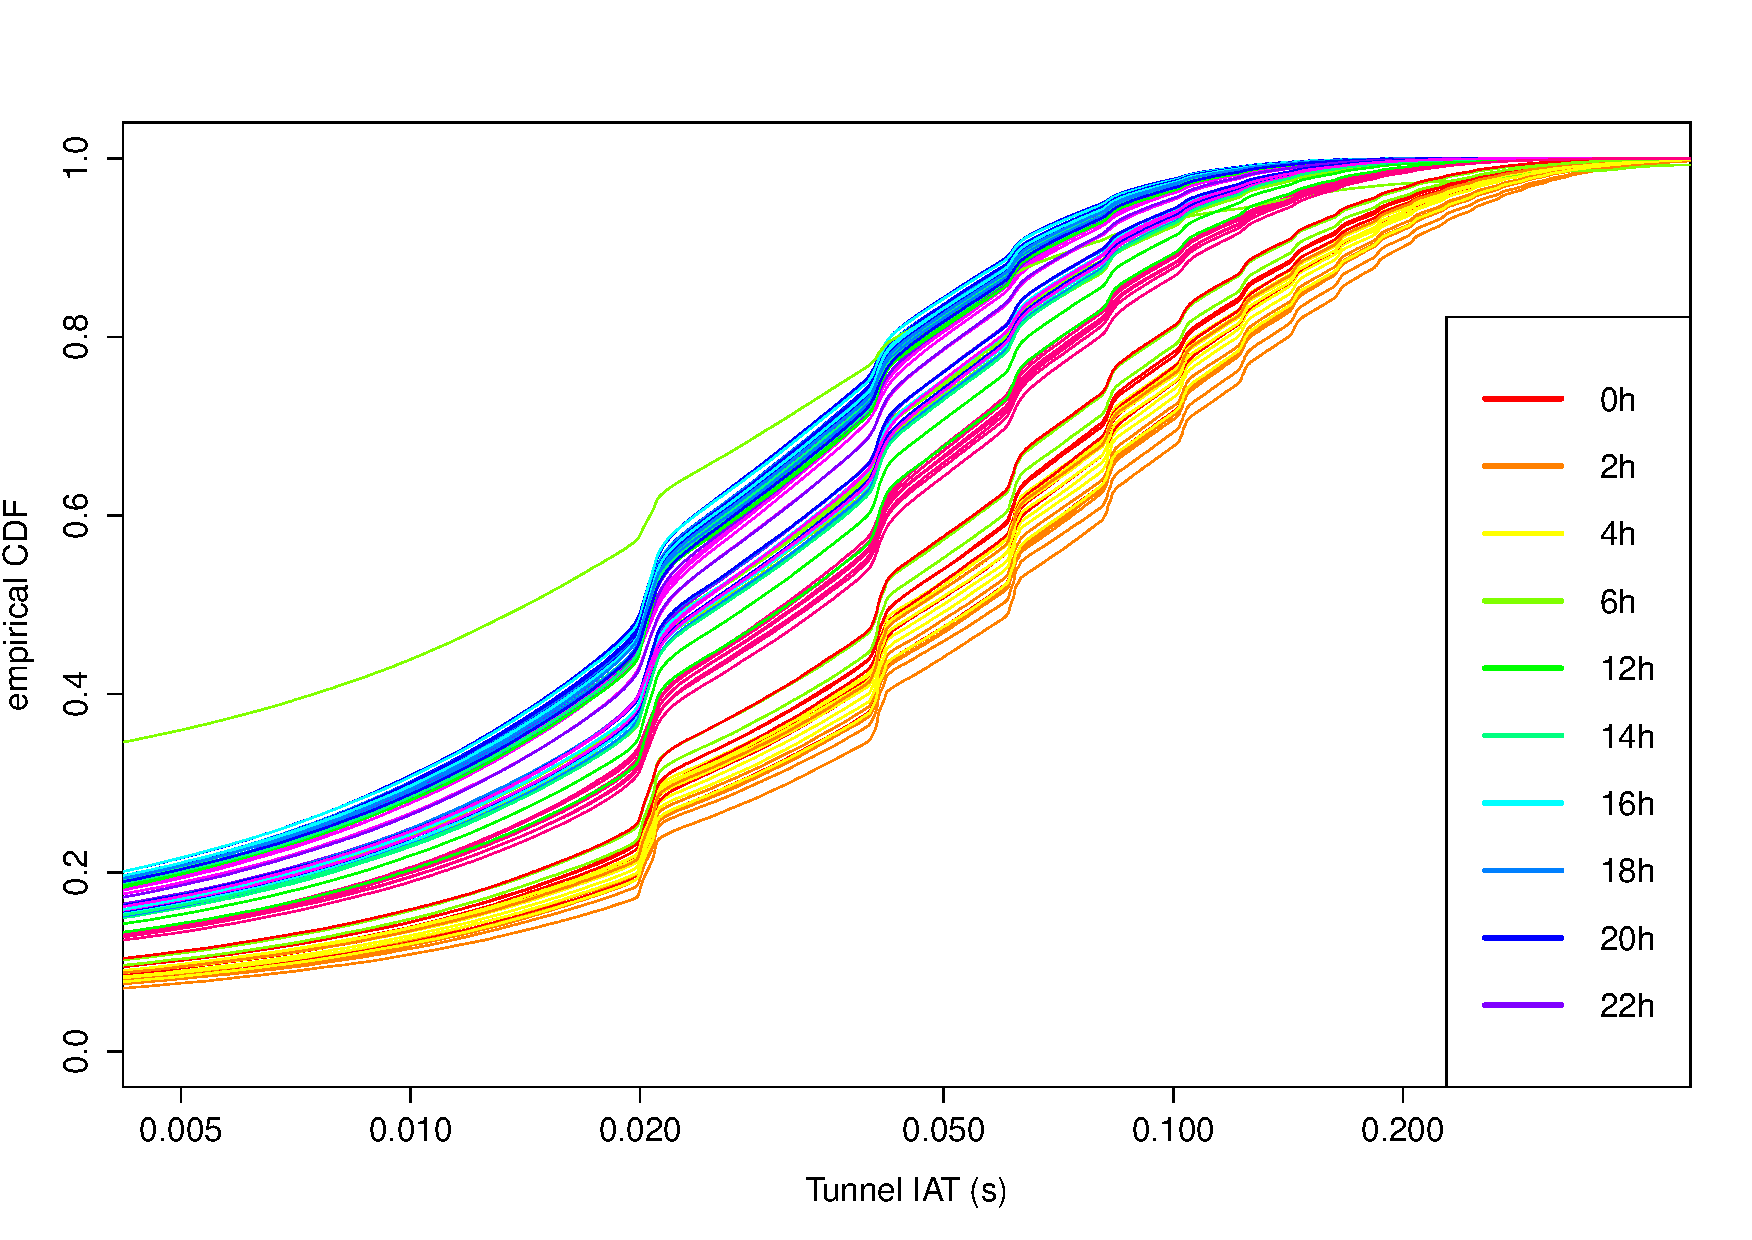
\includegraphics[width=\textwidth]{figures/R-IAT-ecdf-2h-log.png}
        %         \caption{All incoming tunnel requests.}
        %         \label{fig:IAT-ecdf-2h-all}
        % \end{subfigure}%
        %~ %add desired spacing between images, e. g. ~, \quad, \qquad etc.
          %(or a blank line to force the subfigure onto a new line)
        \begin{subfigure}[b]{0.50\textwidth}
            \centering
            \includegraphics[width=\textwidth]{images/qq-total-vs-android.pdf}
            \caption{Android duration over the total duration.}
            \label{c4:fig:qq-total-vs-android}
        \end{subfigure}%
        ~
        \begin{subfigure}[b]{0.50\textwidth}
            \centering
            \includegraphics[width=\textwidth]{images/qq-total-vs-ios.pdf}
            \caption{iOS duration over the total duration.}
            \label{c4:fig:qq-total-vs-ios}
        \end{subfigure}

        \begin{subfigure}[b]{0.50\textwidth}
            \centering
            \includegraphics[width=\textwidth]{images/qq-total-vs-dongle.pdf}
            \caption{3G Dongle duratio over the total duration.}
            \label{c4:fig:qq-total-vs-dongle}
        \end{subfigure}%
        ~
        \begin{subfigure}[b]{0.50\textwidth}
            \centering
            \includegraphics[width=\textwidth]{images/qq-total-vs-smartphone.pdf}
            \caption{Smartphone duration over the total duration.}
            \label{c4:fig:qq-total-vs-smartphones}
        \end{subfigure}
 \caption{Q-Q Plots of the tunnel duration distributions per operating system, with encircled deciles.}
\label{c4:fig:qq-plots}
\end{figure}

In an attempt to show which of the presented categories have an impact on the total duration (if at all), we present Q-Q plots of the various categorized durations against the total duration in Figure~\ref{c4:fig:qq-plots}. In theory, if both durations follow the same distribution, one expects a straight line through the origin at an angle of 45$^o$. A steeper incline indicates less densely spaced values in the distribution at the y axis. Looking at igures~\ref{c4:fig:qq-total-vs-android} and \ref{c4:fig:qq-total-vs-ios} which compare different operating systems, both similar and dispersing parts can be observed. While tunnel durations on Android  are more similarly distributed for the shorter and longer durations, iOS device tunnel durations are most similar to the overall tunnel duration distribution in the middle range of values.

Combining all types of smartphones together and comparing them to the other major player in any mobile network, the 3G dongles, we observe in Figure \ref{c4:fig:qq-total-vs-smartphones} that both the total and the smartphone durations are almost equally distributed (except for minor variations). On the other hand, 3G dongles follow a very different distribution, see Figure \ref{c4:fig:qq-total-vs-dongle}. Their effect on tunnel management signaling seems to be negligible despite the  large amount of traffic they are causing. Therefore, we conclude that planning and dimensioning of the control plane needs to keep smartphone behaviors more closely in mind than that of other device types.


\begin{figure}[htb]
	\centering
	\includegraphics[width=1.0\textwidth]{images/stacked-durations-2-fixed.pdf}
	\caption{Stacked logscale bin plot of the number of tunnels with duration in this bin; classified by Android, iOS and 3G dongles.}
	\label{c4:fig:stacked-durations}
\end{figure}

Figure~\ref{c4:fig:stacked-durations} shows another interesting influence the operating system has on signaling in the mobile core network. This plot shows the relative number of tunnels with a duration in one of 1000 logarithmically scaled bins, stacked by OS category on top of each other. As with the separate distributions, we discover that the durations are not evenly distributed, but rather follow sharp spikes. The largest spike across all categories is the one at a duration of 30 minutes, making up about 1.8\% of all tunnels in the network. Since this spike happens across all device types, we think this makes a rather strong case for being network-induced, and an indication for the aforementioned possible IDLE state transition. On the other hand, the bulk in the short-to-medium ranges of tunnel duration is rather not governed by the two major smartphone operation systems but by other devices in the network, which do not show major spikes in other bins. We can also recognize a long-tail behavior in the distribution of tunnel durations.






%%%%%%%%%%%%%%%%%%%%%%%%%%%%%%%%%%%%%%%%%%%%%%%%%%%%%%%%%%%%%%%%%%%%%%%%%%%%%%%
\subsubsection{\texorpdfstring{\acrshort{gtp}}{GTP} Tunnel Arrivals}

NOTE: IAT cannot be realistically be conducted with categories and still relate to the total system load.

Having characterized the dataset available to us we now shed some light on the control plane and load dynamics in a mobile core network and attempt to show the possible impact of certain devices or other properties of the network. 



While tunnel durations and the involved signaling at the beginning and end of the duration is one aspect of control plane load, the number of tunnel arrivals might be another, which we are looking into in this section.

In addition to describing the arrival process on the basis of the number of arrivals, we also take a look at the tunnel inter-arrival time. Specifically, with this process we mean the arrival of tunnel requests, i.e. GTP CREATE requests, at the \gls{GGSN}. This also adds to the foundation of the load model constructed in the next chapter. 

\begin{figure}[htb]
	\centering
	\includegraphics[width=\columnwidth]{images/create_freq.pdf}
	\caption{Tunnel arrivals in one second intervals.}
	\label{c4:fig:freq-arrivals}
\end{figure}

Figure \ref{c4:fig:freq-arrivals} depicts the number of arrivals per second during the whole weeklong period. Of note is the clear bimodal nature with one peak around twelve and the other in the low thirties. While the distribution is rather compact around these two peaks, there are some clear outliers up to 107.
If we again hypothesize that an increased number of arrivals means higher load in the network, we can assume that load is not constant but rather switches between two modes with some periods with extraordinary load induced by an increased number of arrivals.

\begin{figure}[htb]
	\centering
	\includegraphics[width=\columnwidth]{images/R-createspersecond-1h-violin.pdf}
	\caption{Violin plot of tunnel arrivals in one second per time of day.}
	\label{c4:fig:freq-arrivals-per-second-violin}
\end{figure}

To find the cause of these two modes we take a peek at the diurnal arrival pattern. Figure \ref{c4:fig:freq-arrivals-per-second-violin} contains a violin plot showing again the arrivals per second but broken down by time of day. A violin plot, while being similar to a box plot, additionally shows the density of the individual items on the vertical axis.
The nocturnal median from around midnight to 5am and the longer daytime median, 8am to 19pm, closely resemble the two modes found in the histogram. In between are short transition phases. Notably, during daytime the arrivals and their densities are spread out on a much larger value range. This could be an indication of load fluctuations in the system.


\begin{figure}[htbp]
        \centering
\makebox[\textwidth]{        
        \begin{subfigure}[b]{0.45\paperwidth}    
                \centering
                \includegraphics[width=\textwidth]{images/R-IAT-all-2h-ecdfs.pdf}
                \caption{All tunnel requests.}
                \label{c4:fig:IAT-ecdf-2h-all}
        \end{subfigure}%
        ~
        \begin{subfigure}[b]{0.45\paperwidth}
                \centering
                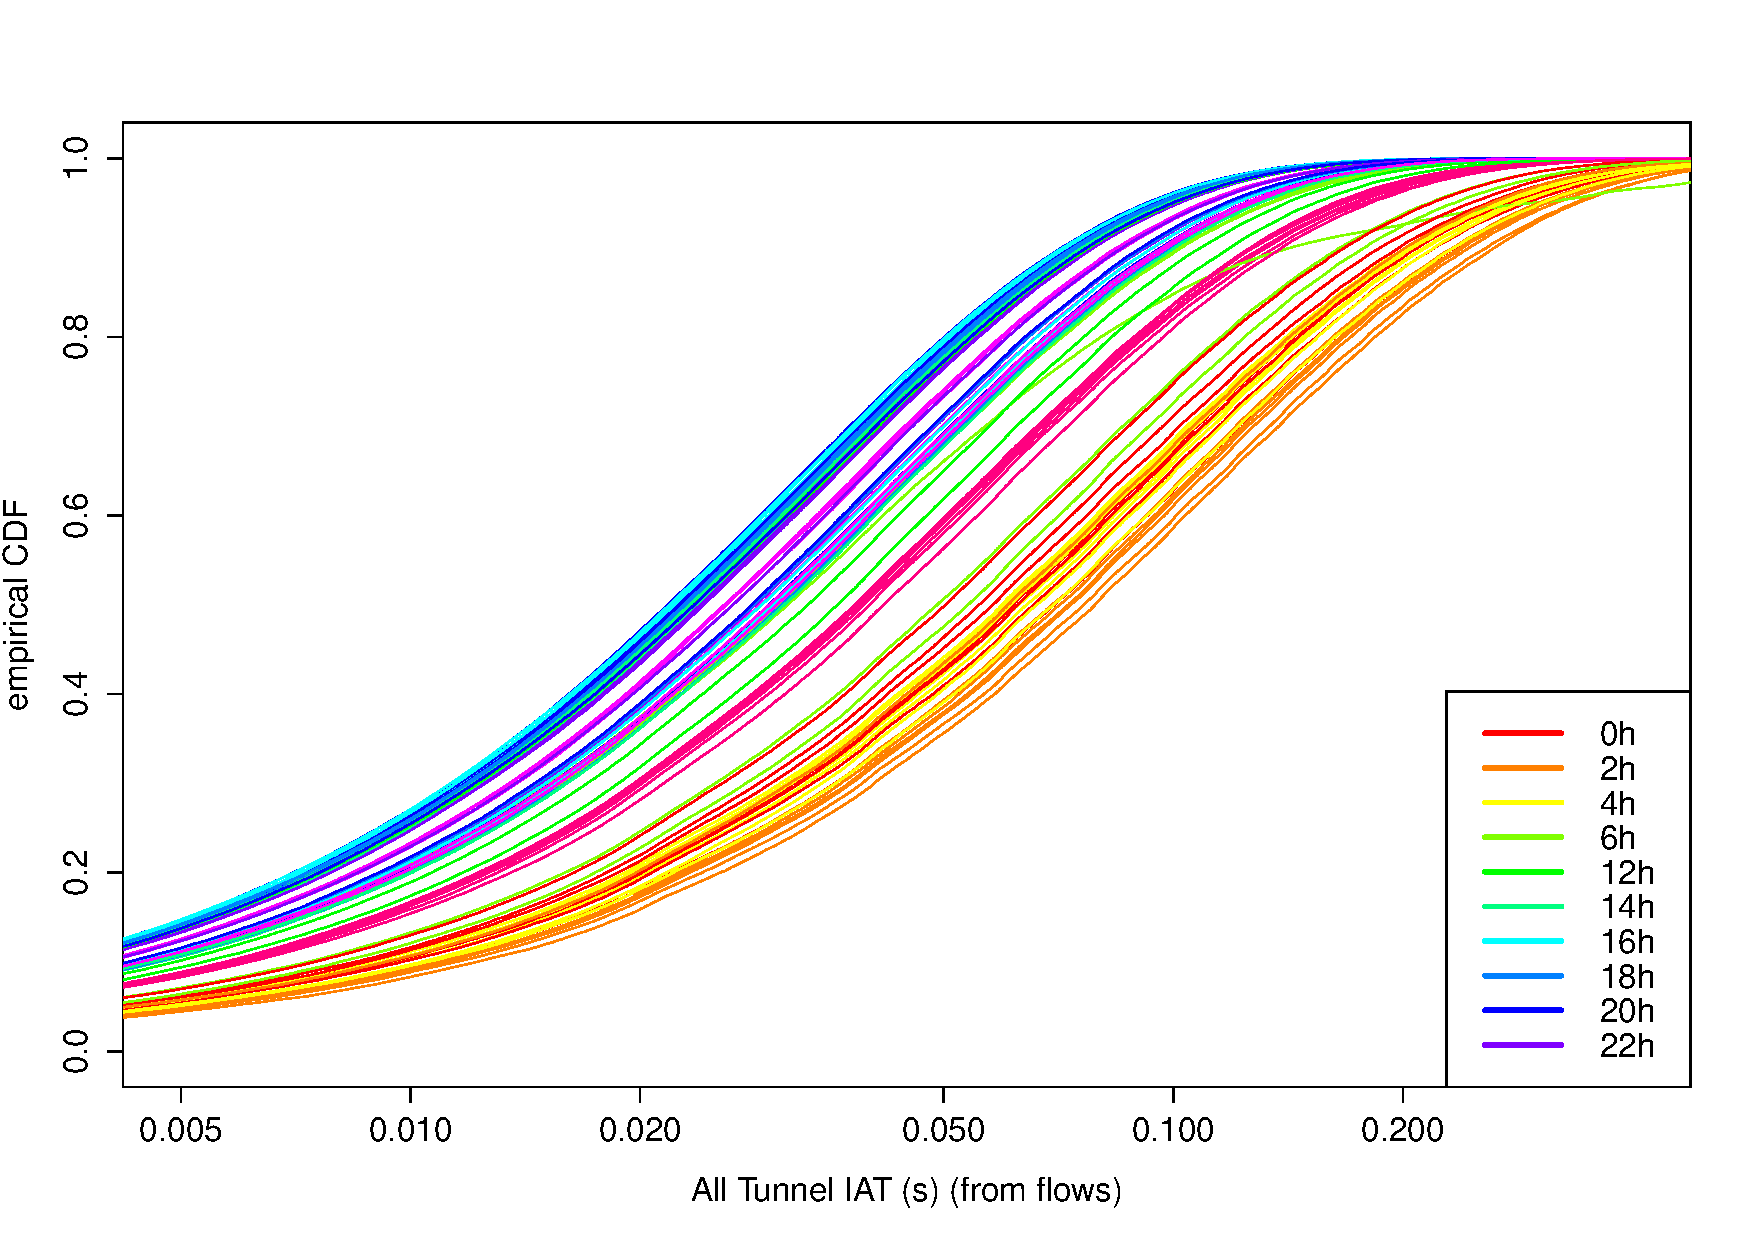
\includegraphics[width=\textwidth]{images/R-IAT-fromflows-ecdfs-2h.pdf}
                \caption{Only tunnels with data flows.}
                \label{c4:fig:IAT-ecdf-2h-active}
        \end{subfigure}
        }

 \makebox[\textwidth]{    
        \begin{subfigure}[b]{0.45\paperwidth}
                \centering
                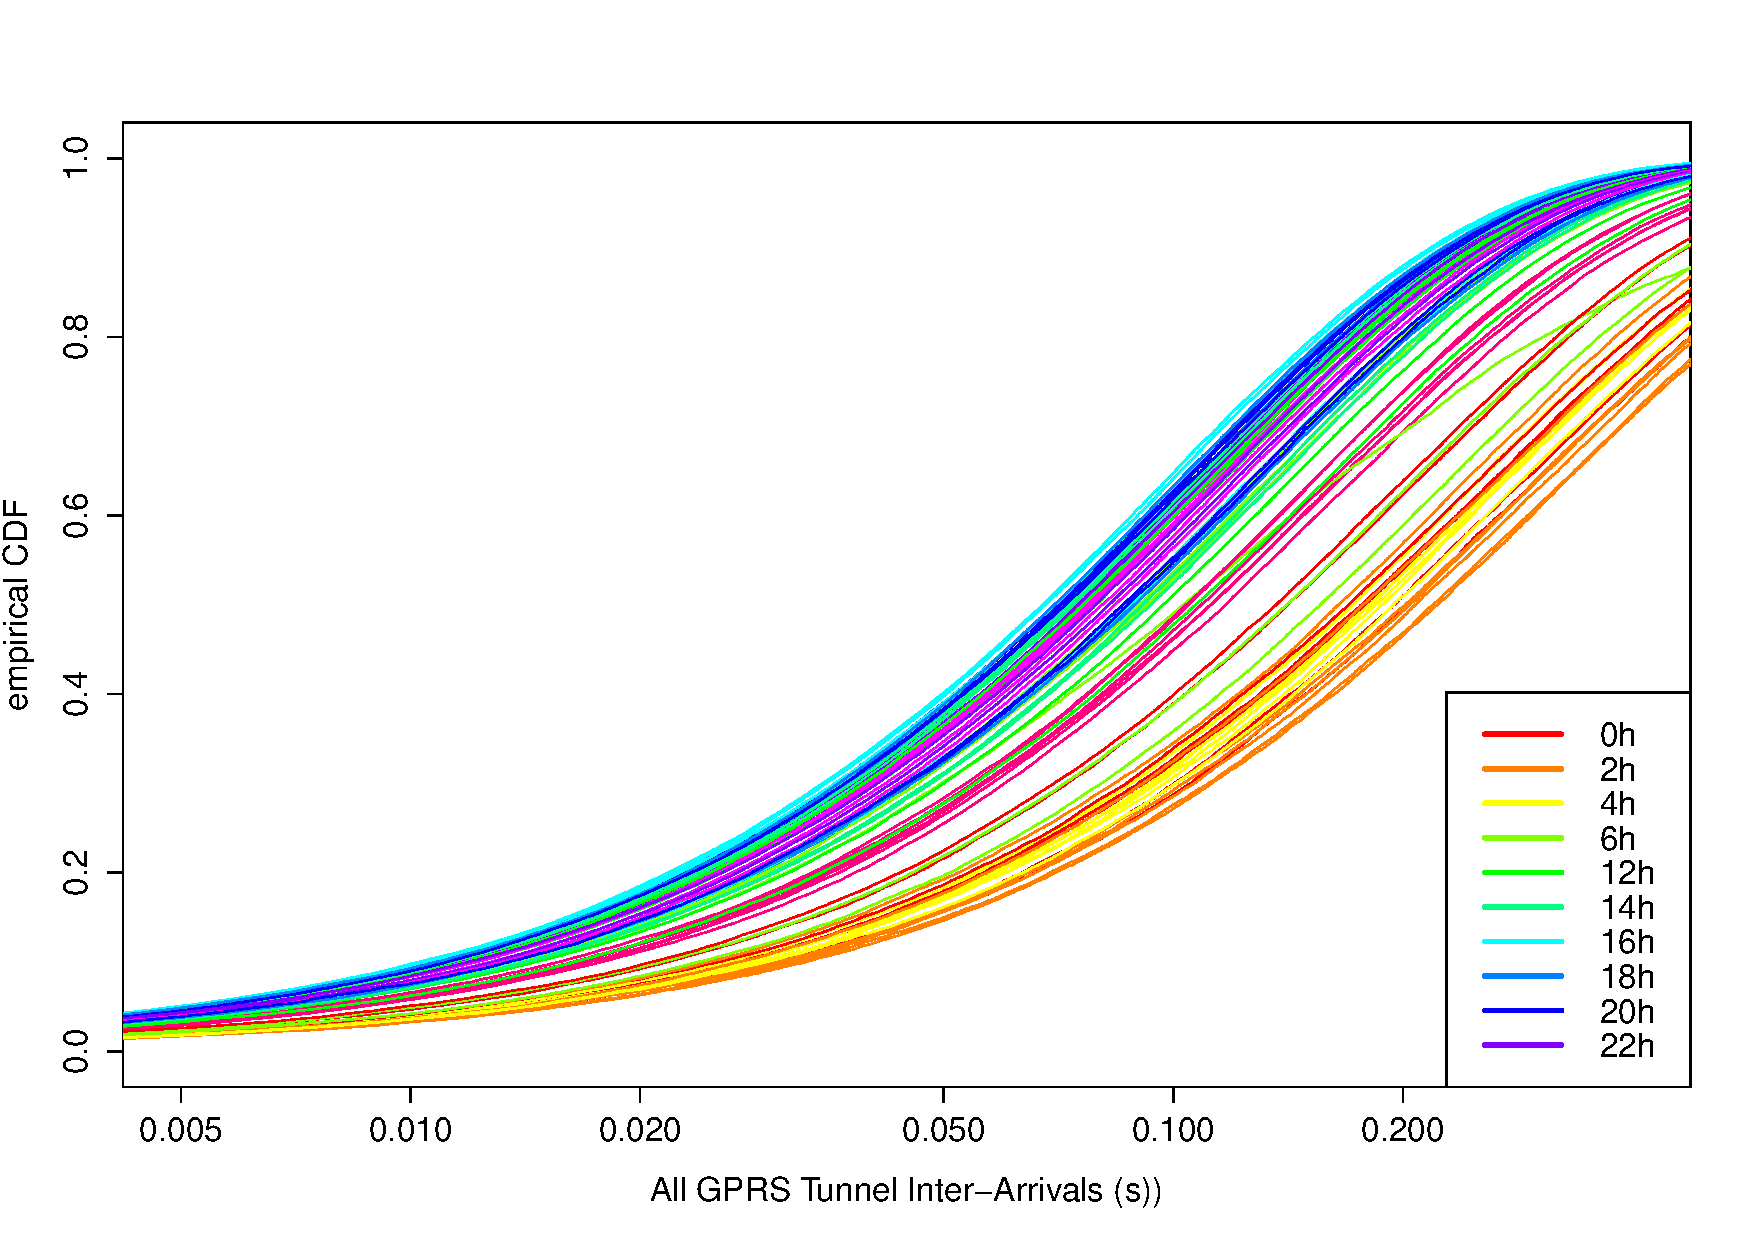
\includegraphics[width=\textwidth]{images/R-IAT-fromflows-gprs-ecdfs-2h.pdf}
                \caption{Tunnels with data flows initiated in GPRS.}
                \label{c4:fig:IAT-ecdf-2h-active-gprs}
        \end{subfigure}%
        ~
        \begin{subfigure}[b]{0.45\paperwidth}
                \centering
                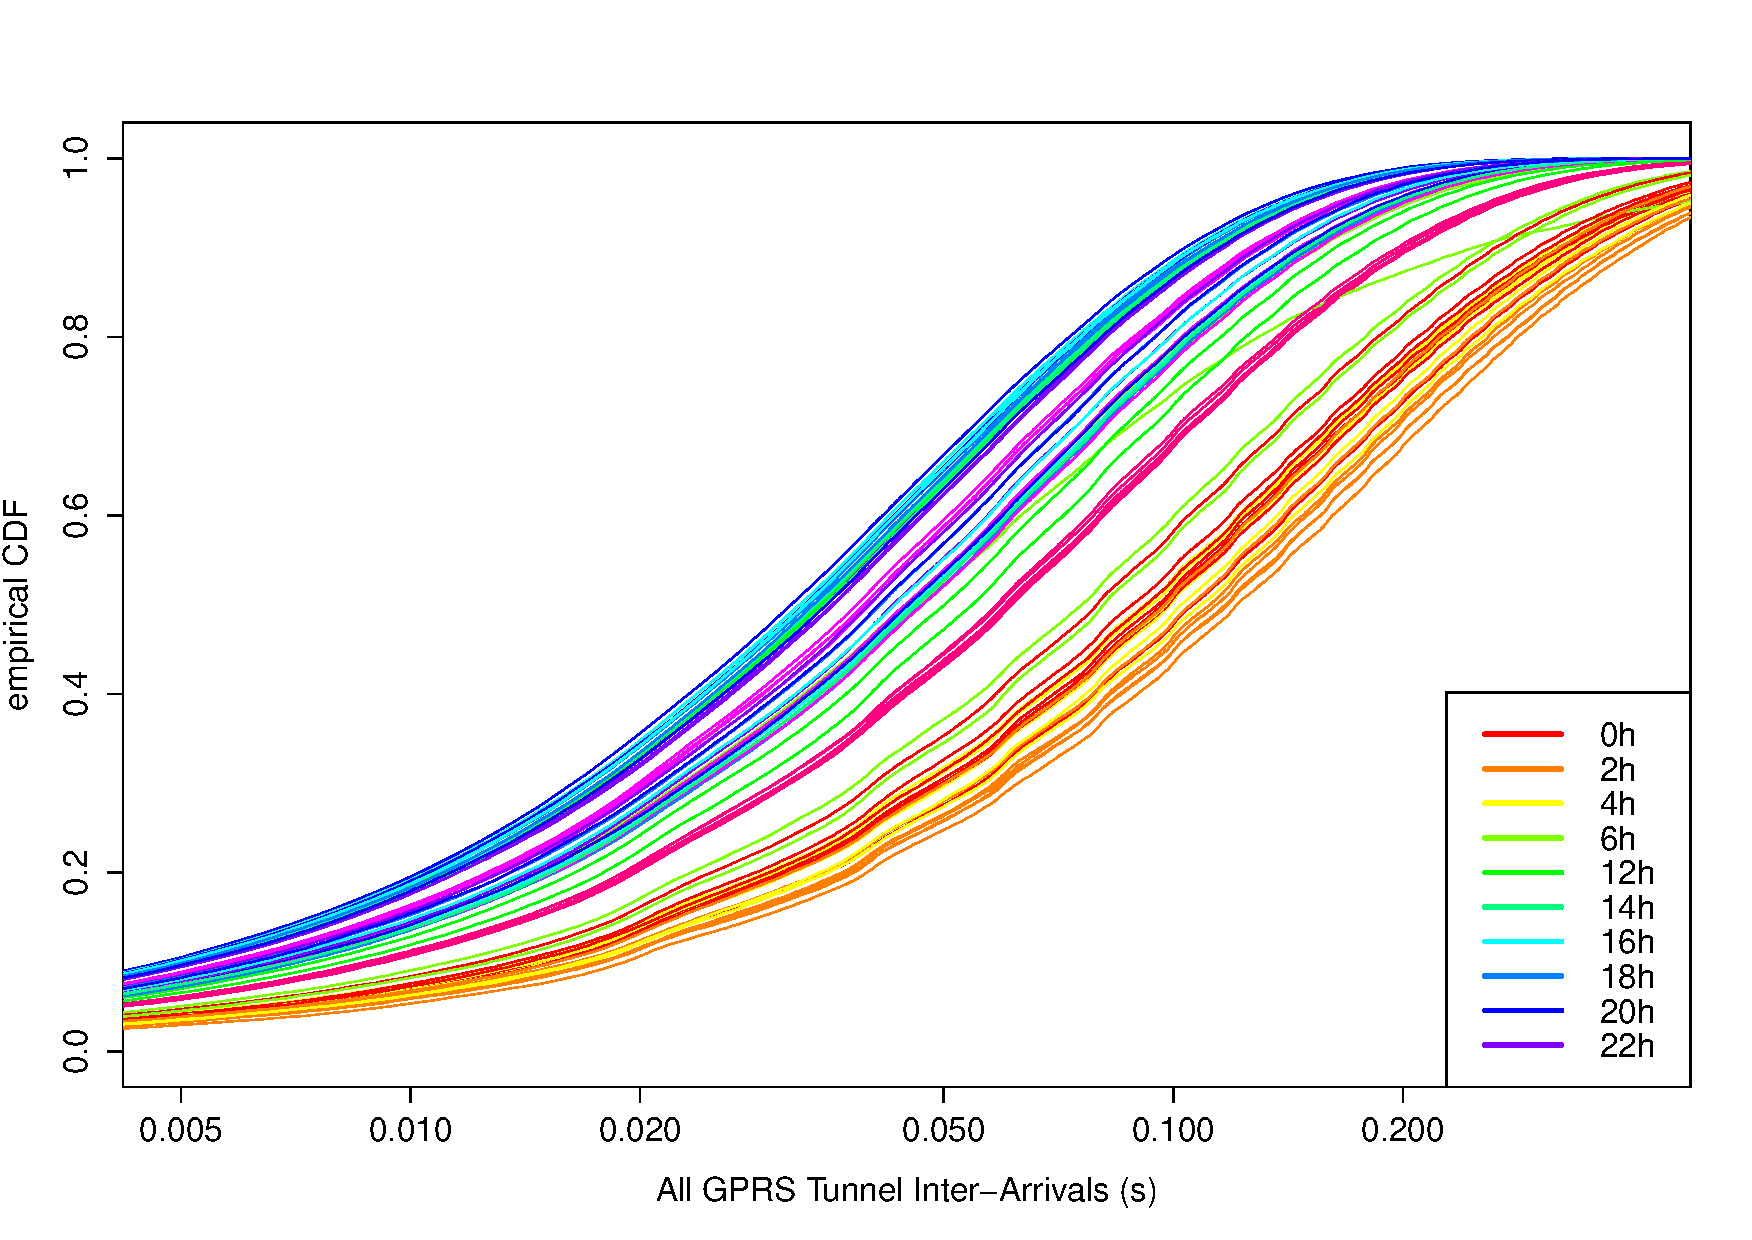
\includegraphics[width=\textwidth]{images/R-IAT-fromflows-umts-ecdfs-2h.pdf}
                \caption{Tunnels with data flows initiated in UMTS.}
                \label{c4:fig:IAT-ecdf-2h-active-umts}
        \end{subfigure}
}
        \caption{Empirical cumulative distribution function of the tunnel inter-arrival time in seconds by time of day for each day of one week.}
        \label{c4:fig:IAT-ecdf-2h}
\end{figure}

To investigate the arrivals from yet another angle we take a look at inter-arrival time of the tunnels in Figure~\ref{c4:fig:IAT-ecdf-2h}. This metric is more suited to describe the arrival process in the toy queuing model we propose. The empirical CDFs are again broken down by time of day, the same diurnal load oscillation can be observed. The medians range between about 20 and 60 milliseconds. Figure~\ref{c4:fig:IAT-ecdf-2h-all}, which represents all tunnel requests that the \gls{GGSN} received, shows wave-like steps in 20ms intervals in the plot. As this is happening very regularly at every time of the day we believe, that this effect must be from a source inside the mobile network and not induced from the outside, .e.g. through mobile devices.

This becomes even more peculiar when further breaking down the tunnel arrivals. We now distinguish between active tunnels, i.e. tunnels, that actually transported user traffic during their lifetime (cf. Fig.~\ref{c4:fig:IAT-ecdf-2h-active}), and active tunnels, which were created while having a GPRS (Fig.~\ref{c4:fig:IAT-ecdf-2h-active-gprs}) or UMTS (Fig.~\ref{c4:fig:IAT-ecdf-2h-active-umts}) connectivity, respectively. Note that only about 86\% of requested and created tunnels where actually used for user data transmissions afterwards. The 20ms-steps occur strongest when observing all tunnel arrivals, in a weaker form it is also present in the active and \gls{UMTS} tunnel portion. 

Our working hypothesis as to the origin of the effect is the \gls{TTI}. This time indicates the duration of a radio transmission and is usually either 10 or 20 milliseconds in length. It is also in sync for the whole network of base stations making the \gls{TTI} noticeable even when not measuring directly at the radio link. The observed step-width of 20ms therefore indicates, that the signaling procedure the GTP CREATE is part of, includes at least one trip from the mobile device over the radio interface. This makes sense, as the tunnel is typically created during the GPRS Attach procedure, which is indeed initiated at the user's device. Unfortunately, this also makes the tunnel arrivals come in somewhat batched, which could momentarily increase the load at the \gls{GGSN} that then would need to process more requests at once than if the arrivals followed a smooth stochastic distribution.




%%%%%%%%%%%%%%%%%%%%%%%%%%%%%%%%%%%%%%%%%%%%%%%%%%%%%%%%%%%%%%%%%%%%%%%%%%%%%%%
\subsection{\texorpdfstring{\acrshort{gtp}}{GTP} Tunnel Event Processing Time}

This brings us to another and potentially more direct measure of \gls{GGSN} load, namely the event processing time, meaning the time it takes for the \gls{GGSN} to fulfill a \gls{gtp} request. This is calculated from the requested and finished timestamps of every \gls{gtp} event in our dataset. As the measurement is conducted at the Gn interface these timestamps represent the time the \gls{gtp} signaling request moves to the \gls{GGSN} and the time the response transitions through the link.

As stated in the previous section, it would be of special interest to know if the setup time of tunnels is influenced by anything, as this is one of the \gls{GGSN}'s most time-sensitive jobs and can impact the time a user has to wait before being able to actually transfer data. Unfortunately, some issues with the dataset did not allow the investigation of the processing time of either create and delete messages.

\begin{figure}[htb]
	\centering
	\includegraphics[width=1.0\textwidth]{images/R-update-time-cdfs.pdf}
	\caption{Empirical CDFs of the time it takes a GGSN to process a GTP update event, plotted for each hour of the day.}
	\label{c4:fig:update-time}
\end{figure}


However, we could investigate the processing time of \gls{gtp} update messages. The core network transmits roughly two orders of magnitude more update than either create or delete events and therefore the number of usable events exceeded the significance level. While no direct investigation of the setup and deletion procedures was possible with these events, a rough overall picture of load can still be attained through this. Figure \ref{c4:fig:update-time} depicts a band of empirical cumulative distribution functions for the processing time of update events broken down by time of day. The processing time is almost uniformly distributed between 2 and 22 milliseconds, with a slightly longer duration during the evening, making for a continuous uniform distribution. This is rather unexpected as uniform distributions do not usually occur in computing processes. According to the central limit theorem one would rather expect to see a normal distribution influenced by, e.g., scheduling or queuing artifacts. In the future we hope to investigate these features more closely, including a proper investigation of the tunnel setup and teardown processing time, if the dataset allows it.



%%%%%%%%%%%%%%%%%%%%%%%%%%%%%%%%%%%%%%%%%%%%%%%%%%%%%%%%%%%%%%%%%%%%%%%%%%%%%%%
\subsection{Statistical Evaluation and Data Fitting}
\label{c4:sec:statistical_evaluation}


\begin{figure}[htb]
  \centering
  \includegraphics[width=0.8\textwidth]{images/R-IAT-active-fit-cdf-facets.pdf}
  \caption{Empirical and exponentially fitted CDFs of the tunnel interarrival duration by time of day. CDFs are overlapping as the coefficient of determination is close to $1$.}
  \label{fig:pdparrivalsecdf}
\end{figure}

Using this dataset, we can obtain the distributions required for the models. At first, we take a look at the tunnel interarrival time in Figure~\ref{fig:pdparrivalsecdf}.
%This can be a good measure for the load a \gls{GGSN} experiences, as every incoming tunnel carries several signaling interactions, processing and state with it.
Typically, a device will only hold one tunnel at a time, but this one tunnel can be initiated and shut down in rapid succession, thus causing the aforementioned issues in the radio network. The arrivals also show a strong diurnal effect, closely resembling patterns present in the actual user traffic: A decline of arrivals, i.e. longer interarrivals, late in the night and during the early morning hours with a peak rate in the afternoon and early evening. To represent this time-of-day dependence in the model, the measurement was split into the four time slots displayed in the figure. Each slot was then fitted with an exponential distribution by way of moments matching. This results in the cumulative distribution function $F(x) = 1- e^{-\lambda x}, x \geq 0$ with $\lambda$ given in Table~\ref{tab:fits} for the four time slots. The fitted functions match the empirical data quite well, with some deviation present at the left tail but overall with a positive correlation coefficient approaching 1.

\begin{figure}[htb]
  \centering
  \includegraphics[width=0.8\textwidth]{images/timeslot-fits.pdf}
  \caption{Empirical and fitted CDFs of the tunnel duration by time of day with fitted rational functions.}
  \label{c4:fig:fittedsdurationlots}
\end{figure}

The second important tunnel property is the duration the \gls{PDP} Context state accompanying a \gls{gtp} tunnel is held at the \gls{GGSN}. Fig.~\ref{c4:fig:fittedsdurationlots} shows the tunnel durations split up for the time of day, as there is once again a slight diurnal effect present, albeit with shifted peaks. Longer tunnels tend to occur at night, shorter tunnels during midday.
%Further properties of the tunnel duration, especially the correlation with device types and operating systems, were already investigated in detail in our previous work \cite{metzger2012research,metzger2013}.
For the model, a distribution fit of the tunnel duration was also desired. However, none of the basic probability distributions (including exponential, gamma, and Weibull distributions) fit the tunnel duration well enough. One of the reasons for this probably being the correlation of the tunnel duration to a large number of factors, including user behavior and network-specific timers and procedures,
%Tunnels are shut down by the network after specific events (e.g. a 30-minute idle timer), 
introducing artifacts which make it hard to fit any distribution against. Instead, we fitted rational functions to the empirical CDF using Eureqa \cite{eureqa_paper, eureqa_software}. This allowed for a much closer fitting while still smoothing out some of the artifacts. Table~\ref{tab:fits} also displays these functions fitted to the inverse CDF, to be directly used for generating random numbers using the inversion method. Both the CDF in Fig.~\ref{c4:fig:fittedsdurationlots} as well as the Pearson correlation coefficient confirm the goodness of the fitted functions.


\begin{table}[htb]
  \caption{Parameters for the exponentially distributed inter-arrival times and corresponding Pearson correlation coefficients; also contains the inverse functions fitted to the empirical duration distribution and correlation coefficients of the fit.}
  \label{tab:fits}
  \tabulinesep=1.2mm
  \centering
\begin{tabu}{X[0.9,l]X[r]X[r]X[4.5,r]X[r]} 
  \toprule
  \textbf{Time of Day} & $\mathbf{\lambda}$ & $\mathbf{R_{arrival}}$ & \textbf{Inverse Fitted Duration Function} & $\mathbf{R_{dur}}$\\ 
  \midrule
  0h-5h & $10.67477$ & $0.99538$ & $0.919208 - 60.6136y - 3498.78y^3 - \frac{110.707y + 2289.94y^3}{y - 1.00469}$ &  $0.9999021$ \\
  6h-11h & $24.53298$ & $0.99216$ & $1 + 117.484y - 368.643y^2 - \frac{1720.13y^4}{y - 1.0041}$ & $0.9998909$ \\
  12h-17h & $29.2504$ & $0.99256$ & $0.952566 + 69.4907y + \frac{81146.1y^3 + 1.08572\times10^6y^5}{805 - 802.01y}$ & $0.9999027$ \\
  18h-23h & $23.49983$ & $0.98617$ & $0.911924 + 82.0562y - \frac{2936.93y^4}{1.94468y - 1.9532}$ & $0.9998071$ \\
  \bottomrule
\end{tabu}
\end{table}




%% to be integrated into evaluation
\begin{figure}[htb]
  \centering
  \includegraphics[width=1.0\textwidth]{images/R-duration-activetunnels-hours-ecdf.pdf}
  \caption{Tunnel duration of all active tunnels by time of day.}
 \label{c4:fig:duration-timeofday-ecdf}
\end{figure}





% \begin{table}
% \centering
% \caption{TAC Statistics}
% \begin{tabu}{|X|X|X[1.5]|X|X|X|} \hline
% & \textbf{\# of Flows} & \textbf{Total Traffic (Bytes)} &  \textbf{\# of Tunnels} & \textbf{\# of GTP Signalling Msgs} & \textbf{\# of Distinct IMSIs}\\ \hline
% Total          & 2234659247 & 122758578593993 (112TB)    & 16632094 & 409733865 & 1255293 (all) / 1030895 (with flows) \\ \hline
% In TAC DB      & 2228315260 & 122716712007150 (111.61TB) & 14565430 & 372662108 & 1015891 \\ \hline
% Smartphones    & 459990512  & 15721818747754 (14.30TB)   & 10030734 & 311342846 & 476675  \\ \hline
% Regular phones & 5705832    & 448140315058 (0.41TB)      & 897529   & 3860162   & 116124  \\ \hline
% 3G dongles     & 1487230062 & 92215931895630 (83.87TB)   & 2114756  & 39053819  & 315003  \\ \hline
% Android        & 241973565  & 7953178401958 (7.2TB)      & 2383255  & 177537567 & 175919  \\ \hline
% iOS            & 161408903  & 5481693567152 (5TB)        & 3145384  & 83374590  & 99679   \\ \hline
% Symbian        & 22827418   & 1332996529271 (1.21TB)     & 3520242  & 18479002  & 162790  \\ \hline
% Blackberry OS  &            & 128074907884 (0.12TB)      &          &           &         \\ \hline
% \end{tabu}
% \end{table}


%Devices with GTP signaling but no user plane traffic: (\#distinct imsis gtp db)-(\#distinct imsis flow db):
% $255293-1030895=224398\text{ or }17.88\%$

%%%%%%%%%%%%%%%%%%%%%%%%%%%%%%%%%%%%%%%%%%%%%%%%%%%%%%%%%%%%%%%%%%%%%%%%%%%%%%%%
%\subsection{Correlations to User Traffic}
% TODO, incl. measurements



%%%
% Direct signaling traffic overhead in relation to user traffic and induced network load

% GTP Header: 12 Byte
% IE header and footer: 2 Byte
% Maximum minimum data size including all \glspl{IE}: 221 Byte + 12 Byte Header + 2*37 Extension Header = 307 Byte
% Minimum size of message with just mandatory \glspl{IE}: 12 + 30 + 2*5 = 52 Byte

% 307 Bytes:
% calculation from our dataset
% Total maximum signaling traffic with this calculation: 117.15GB
% Ratio: 0.10\%
% 52 Bytes:
% Total maximum signaling traffic with this calculation: 19.84GB
% Ratio: 0.02\%
% Total traffic: 122758578593993


% signaling calc:
% gtp signaling traffic volume estimation $v_s$ = (1059B gtp message + 8B udp header + 20B ipv4 header) = 1087B * 409733865 number of request/response pairs * 2 (2 messages per pair) = 8,9076142E11B
% ratio to total $r=\frac{v_s}{v_t}=0.72\%$  $v_t=122758578593993B$




%%%%%%%%%%%%%%%%%%%%%%%%%%%%%%%%%%%%%%%%%%%%%%%%%%%%%%%%%%%%%%%%%%%%%%%%%%%%%%%%
%!TEX root = ../../dissertation.tex
%%%%%%%%%%%%%%%%%%%%%%%%%%%%%%%%%%%%%%%%%%%%%%%%%%%%%%%%%%%%%%%%%%%%%%%%%%%%%%%
\section{Modeling Mobile Network Load}
\label{c4:modeling}

Drawing conclusions from statistical analysis alone is a difficult task. The next logical step lies therefore in the creation of models abstracting this real system, making them easier to calculate with the loss of some precision. This and future improved models should support network operators in predicting the signaling load in their core network with the benefit of improved network engineering and correctly scaling core components.


%%%%%%%%%%%%%%%%%%%%%%%%%%%%
% intro part from MMB 2014
%\section{Introduction}

With the increased importance of smart phones, mobile networks are currently experiencing rapid growth.
Compared to a fixed access provider additional aspects have to be taken into account when dimensioning a mobile network. 
First and most prominent is the planning of radio access cells --- their coverage, frequency selection,  and backhaul, i.e. connection to the operator's network. Aside from substantial administrative and financial efforts this problem has been largely solved, radio network planning tools and research readily exists \cite{tutschku1998demand}.
Albeit of equal importance, there is much less public knowledge and research on the second aspect in setting up the mobile network: dimensioning the core network. Consisting of a large number of specialized network nodes not available as of-the-shelf commodity hardware and in need of careful tuning to each other, correctly putting together the core is no small feat. Unlike fixed access, mobile access networks require much more state to be held, with the nodes having to signal any state-change throughout the network.

One major metric to consider in the dimensioning is the number of supported tunnels, i.e. connections to the Internet, of the \gls{GGSN}.
The performance requirements of the \gls{GGSN} depend on factors like customers to serve, applications in the network, user behavior and devices used. These factors are, during dimensioning, either unknown or subject to change as user behavior evolves.
But these network components are sold as static middleboxes and cannot not be easily extended with of-the-shelf hardware in order to account for new requirements.
The newly introduced concept of \gls{NFV} \cite{nfv_whitepaper} suggests to harness technologies from cloud computing in the network. This would allow network operators to scale out, i.e. using additional low performance machines, instead of scaling up, which requires them to replace existing hardware with more powerful components.

The contribution of this work is threefold. First, we introduce models for both a traditional \gls{GGSN} as well as a virtual \gls{GGSN} using \gls{NFV}. Secondly, we provide distributions for \gls{gtp} tunnel interarrival times and durations, readily to be used in other studies. Finally, we study performance trade-offs when using a virtual \gls{GGSN}, discussing different options to consider when using a virtual \gls{GGSN}.


%%%%%%%%%%%%%%%%%%%%%%%%%%%%%%%%%%%%%%%%%%%%%%%%%%%%%%%%%%%%%%%%%%%%%%%%%%%%%%%
\subsection{Creating a Simple Toy Queuing Model}

\begin{figure}[htb]
	\centering
	\includegraphics[width=\columnwidth]{images/GGn-model.pdf}
	\caption{Simple toy-model for tunnel-induced load on the core network.}
	\label{c4:fig:ggn-model}
\end{figure}

To begin the modeling process we attempt to represent the tunnel management as a queuing system, specifically as a G/G/n-0 system in Kendall's notation. Figure~\ref{c4:fig:ggn-model} shows this model for the case of our proposed tunnel load metric. Here, tunnels enter the system by a general random distribution, are then ``served'' at the \gls{GGSN} for the duration of their existence, which also follows a general distribution, and leave the system, i.e. are torn down, afterwards. If the serving units are filled, blocking occurs and arriving tunnel requests are rejected.

In this case ``servers'' correspond to available resources at one or more \gls{GGSN}, making the maximum number of tunnels hard to guess and depend on a number of factors. This could include soft-limits like the specific configuration, and hard-limits, e.g. the \gls{GGSN}'s processing and memory constraints. Unfortunately, all of these are unknown to us. Moreover, as the tunnels are all served on a relatively small number of hardware entities they are not independent of each other. Increasing load could very well influence both the arrival as well as the serving process.

For the purpose of creating a toy model we are further simplifying the G/G/n-0 to a M/M/$\infty$ queue. As stated, no actual limit to the number of virtual servers is known and the data also does not show any obvious limits. So we can safely assume an unlimited system and do not have to treat blocking or queuing explicitly.

\begin{figure}[htb]
	\centering
	\includegraphics[width=\columnwidth]{images/R-IAT-ecdfs.pdf}
	\caption{Sampled inter-arrival time CDF and fitted theoretical distributions.}
	\label{c4:fig:IAT-cdfs}
\end{figure}

Furthermore, we fitted univariate distributions to the experimental data for the tunnel inter-arrivals and durations and tested the goodness of the fit both numerically, using Pearson's $\chi^2$ test, and visually for the density and CDF plots. No standard random distribution reaches the significance level for either process. We attribute this fact largely to the various artifacts in the data, e.g. the described wave effect every 20 milliseconds in the inter-arrival time. Matching them visually (confer also the cumulative distribution function plot in Figure~\ref{c4:fig:IAT-cdfs}) we find that the exponential fit is reasonably close to the experimental data in both the arrival and duration cases. Again, these distribution fits are just for a toy model to lay the groundwork for future and improved modeling.


\begin{figure}[htb]
	\centering
	\includegraphics[width=\columnwidth]{images/markovchain.pdf}
	\caption{Markov chain model for the tunnel serving process.}
	\label{c4:fig:markovchain}
\end{figure}

Now, assuming both a Poisson arrival and an exponential serving process, a Markov chain representing the queue can be set up (cf. Fig.~\ref{c4:fig:markovchain}) and stationary analysis can be conducted. From the measured data an arrival rate of $\lambda=25.64123$ and the parameter $\mu=0.0001586728$ for the exponential service time distribution are calculated. Using Little's Law this gives an estimate for the mean number of concurrent tunnels at the \gls{GGSN} of 

$$
L=\frac{\lambda}{\mu}\approx 161\,599. %=161598.14.
$$

As stated, the amount of state held at the node and propagated through the network is directly related to the number of tunnels. Therefore, we propose this metric as an initial estimate of the load at the \gls{GGSN}.


%%%%%%%%%%%%%%%%%%%%%%%%%%%%%%%%%%%%%%%%%%%%%%%%%%%%%%%%%%%%%%%%%%%%%%%%%%%%%%%
\subsection{Advanced Models} 


On the basis of this toy model better fitting models can now be constructed. Those should also factor in more of the core network's properties and specified parameters omitted in this model. Specifically, this means shifting from M/M/$\infty$ to the more generalized G/G/n and therefore finding better distribution fits for the involved processes.

It is also entirely possible that the single queue approach is not the best way to describe control plane load. Several load influencing factors discussed earlier have direct influence on the tunnel arrivals and duration, e.g. the device type or the radio access technology. Therefore, amongst others multidimensional queuing networks or fluid flow could be a better fit. Our plan is to conduct further investigations into the modeling of mobile core network signaling. This also includes a rough simulative approach, which could also be used to validate our models against experimental data.


%%
\subsubsection{Monolithic \texorpdfstring{\acrshort{GGSN}}{GGSN}}

In this section we provide a model for a traditional \gls{GGSN} and discuss a model for a virtual \gls{GGSN} using \gls{NFV}. In \gls{NFV} \cite{nfv_whitepaper} static network middleboxes are replaced by commodity hardware. The tasks solved by the original middleboxes are then solved by dediciated software.

\begin{figure}[htb]
  \centering
  \includegraphics[width=0.6\textwidth]{images/ggsn-monolithic.pdf}
  \caption{Model of a Traditional GGSN}
  \label{fig:model_traditional_ggsn}
\end{figure}

First, we give a model for a \emph{traditional} \gls{GGSN}, i.e. a network static network component.
While we consider the \gls{GGSN} to be one fixed entity, it can in reality consist of multiple servers. However, due to the fact that the \gls{GGSN} is purchased from a vendor as a middlebox, idle servers can be neither deactivated nor reused for other purposes.

The queuing theory equivalent is displayed in Figure~\ref{fig:model_traditional_ggsn}. New tunnels requests arrive according to a Poisson distribution with a rate of $\lambda(t)$ at the GGSN. This server will have a maximum tunnel capacity of $c_c$. When it is reached, blocking will occur and newly incoming tunnels are rejected. Traditionally, \glspl{GGSN} can be expected to be overdimensioned in such a way, that this rarely happens. If the new tunnel is accepted, it will occupy one of the serving units of the unit for the duration $\mu(t)$ of the tunnel. As stated earlier, we can not model the tunnel duration to be markovian, resulting in a  M/G/$c_c$ loss system. In order to give quality of service guarantees the network operator is interested in the system's blocking probability $p_B$, which we consider to be a key metric of our model. Additionally, the previously described diurnal patterns can are also be modeled by adjusting the arrival and serving process distributions for each time of day. This alternatively also allows just to investigate the busy hour and thus the system's peak load.


%%
\subsubsection{\texorpdfstring{\acrshort{GGSN}}{GGSN} using Network Function Virtualization}
\label{c4:sec:virtual_ggsn}

\begin{figure}[htb]
  \centering
  \includegraphics[width=0.7\textwidth]{images/ggsn-virtualized.pdf}
  \caption{Model of a GGSN using Network Function Virtualization}
  \label{c4:fig:model_nfv_ggsn}
\end{figure}

In the second model, we introduce concepts from \gls{NFV}, i.e. the idea to replace middleboxes with commodity hardware. This allows us to realize benefits from cloud computing, as we are now able to scale out, instead of up. The assumptions of the Markov arrival process $\lambda(t)$ and the serving time distributions $\mu(t)$ are carried over. However, instead of one server processing every tunnel, this model assumes that there are up to $s_{max}$ virtualized servers $s_i$. Each of these is much smaller than the traditional GGSN, having a tunnel serving capacity of $c_i \ll c_c$ and a total system capacity of $c_{max} = s_{max} \times i$.

In its initial state, for efficiency, all but a small portion of the server instances should be shut of. Only, when a certain condition is reached, a new one is provisioned. As a simple example, one could always hold one instance in reserve for upcoming requests and provision as soon as the reserver gets used. Similar rules should apply in the shutdown of servers and should form a hysteresis together with the boot condition. For example it would be possible to keep at least one server in reserve but never more than two.

If these conditions are not carefully selected and are in tune with the expected boot time of an instance, additional blocking can occur. Despite not having reached its maximum capacity, this system will still reject tunnel requests during the provisioning phase when no tunnel slots are free. This could be remedied by a request queue. However, this might just make the system more complex without providing real benefit, as mobile devices usually will repeat their attempts and would time out anyway when the request is taking too long. 

To place incoming tunnel state on one of the available servers a load balancer is required. To ensure, that the system in run time can scale down to its actual needs, the balancer should place tunnels on servers, that are the fullest, keeping the reserve free. It may even migrate tunnel state from almost empty servers away so that these can be shut down, when the condition is fulfilled. Keeping instance close to their capacity should also have no impact on the performance a mobile device associated to a specific tunnel experiences. Adequate strategies for both load balancing and migration will be considered in future work.




%%%%%%%%%%%%%%%%%%%%%%%%%%%%%%%%%%%%%%%%%%%%%%%%%%%%%%%%%%%%%%%%%%%%%%%%%%%%%%%
\subsection{Simulative Validation} 


%%
\subsubsection{Testing the Model Numerically}
\label{c4:sec:model-numerical}

We implement the models using a \gls{DES} with the SimPy \cite{simpy} package as foundation. Our implementation is also publicly available\footnote{\url{https://github.com/fmetzger/ggsn-simulation/}} as a reference for future publications. To be in line with the measurement data we consider a simulation time of 7 days for all simulation scenarios, with a transient phase of 60 minutes accounted for. Ten replications of each scenario were performed. All error bars given in this section show the $5\%$ and $95\%$ quantiles of all replications.


We use the measurements in order to dimension a traditional \gls{GGSN} as a baseline for all further studies. Based on these results, we examine the effects of network function virtualization by scaling \emph{out} instead of up through a virtual \gls{GGSN} model. Finally, we arrive at a more realistic version of the virtual \gls{GGSN} by taking the start up and shut down times into account.


%%
\subsubsection{Queuing Simulation Implementation}


%%
\subsubsection{Traditional GGSN}
\label{c4:sec:eval_traditional_ggsn}

With the help of the interarrival times and duration of tunnels we study the traditional \gls{GGSN} model previously introduced. Whilst our measurements provided us with information on the frequency of new tunnels and the duration they remain active, we have no reliable information on the number of active tunnels the \gls{GGSN} can support. Thus, in a first step, we dimension the \gls{GGSN} in such a way that a suitable blocking probability $p_B$ can be achieved.

\begin{figure}[htp]
  \centering
    \includegraphics[width=1.0\textwidth]{images/traditional-blocking.pdf}
  \caption{Impact of the number of supported parallel tunnels on the blocking probability for the traditional \gls{GGSN} model. For each scenario the mean of all simulated replications as well as $5\%$ and $95\%$ quantiles as error bars are shown.}
  \label{c4:fig:traditional_blocking}
\end{figure}

In Figure~\ref{c4:fig:traditional_blocking} the maximum number of tunnels $n$, that can be active simultaneously, is gradually increased to study the impact on the blocking probability $p_B$. We observe, that as the number of supported parallel tunnels increases, the blocking probability decreases. For the normalized interarrival no blocking is occurring if we allow for more than $5000$ parallel tunnels. Thus, we consider the range of $4000$ to $5000$ parallel tunnels to be of special interest for the remainder of the study.


%%
\subsubsection{Virtual \texorpdfstring{\acrshort{GGSN}}{GGSN}}
\label{c4:sec:eval_ideal_virtual_ggsn}

In order to study the feasibility of the virtual \gls{GGSN} approach discussed in Sec.~\ref{c4:sec:virtual_ggsn}, we compare the performance indicators of the virtual \gls{GGSN} with that of a traditional \gls{GGSN}. To this end, the virtual \gls{GGSN} is simulated in varying configurations.
The number of servers and supported tunnels per server is chosen in such a way that the results can be compared with those obtained from our study of the traditional \gls{GGSN}. Due to simulation time constraints, only a representative subset of scenarios is simulated.

In the virtual \gls{GGSN} model, servers are activated and deactivated on demand, while in the traditional \gls{GGSN} model, the single server is always on. For this investigation a conservative start up and shut down time of \SI{300}{\second} is chosen. Generally, deactivating server instances reduces energy consumption and frees up inactive servers for other use. For this reason, the number of active servers is a relevant performance metric in the virtual \gls{GGSN} model.


\begin{table}[htp]
	\caption{Manipulation check for the experimental factors based on one-way ANOVA.}
	\centering
	\label{c4:tab:manipulation2color}
	\begin{tabu}{X[l]X[r]X[r]X[r]XX}%{lrrrcc}
	\toprule
	& \multicolumn{1}{c}{$F(2,1275)$} & \multicolumn{1}{c}{$\eta^2_p$} & \multicolumn{1}{c}{$p$} & Cohen's & Cohen's\\ 
	&  & & & $f^2$ & $\hat{\omega}^2$ \\ 
	\midrule
	\emph{blocking probability}  & & & & &\\ 
	maxTunnels &  15601.534 & \textcolor{red}{0.993} & $<0.001$ & \textcolor{red}{26.739} & 0.964\\ 
	maxInstances &  10218.173 & \textcolor{red}{0.986} & $<0.001$ & \textcolor{red}{1.068} & 0.516\\ 
	startstopDuration &  0.868 & \textcolor{black}{0.003} & $0.482$ & \textcolor{black}{0.000} & 0.000\\ 
	\midrule
	\emph{mean number of tunnels}  & & & & &\\ 
	maxTunnels &  20448.347 & \textcolor{red}{0.994} & $<0.001$ & \textcolor{red}{27.712} & 0.965\\ 
	maxInstances &  13348.251 & \textcolor{red}{0.989} & $<0.001$ & \textcolor{red}{1.064} & 0.515\\ 
	startstopDuration &  2.872 & \textcolor{black}{0.009} & $0.022$ & \textcolor{black}{0.000} & 0.000\\ 
	\bottomrule
	\end{tabu}
\end{table}

In order to analyze the influence of the different model parameters on the performance metrics, we perform a one-way ANOVA analysis with the results in Table~\ref{c4:tab:manipulation2color}. High values for $\eta_p^2$ and Cohen's $f^2$ \cite{stats} indicate that the main influence for both blocking probability and mean number of tunnels is the maximum number of tunnels $n$ and servers $S_{\max}$, i.e. the total number of possible concurrent tunnels in the system.
Therefore, we study these parameters first.

\begin{figure}[htb]
  \centering
  \includegraphics{images/instanceuse-multiserver-real.pdf}
  \caption{Impact of the maximum number of tunnels and number of servers on number of active servers in the virtual \gls{GGSN} model.}
 \label{c4:fig:instance_use_virtual}
\end{figure}

In Figure~\ref{c4:fig:instance_use_virtual} the \gls{CDF} of the number of active servers for four different virtual \gls{GGSN} configurations is displayed. We observe, that increasing the number of supported tunnels per server allows a larger percentage of servers to be shutdown or used for other tasks. This demonstrates the scaling capability of the virtualized model quite well. Note, that both the scenario with 30 servers and 150 maximum tunnels per server as well as the scenario with 60 servers and 75 maximum tunnels per server share the same maximum amount of tunnels, 4500, being right at the center of the interesting range of candidates.


\begin{figure}[htb]
  \centering
  \includegraphics{images/blocking-comparison.pdf}
  \caption{Relative increase of blocking probability on the number of servers compared to the traditional \gls{GGSN}; with the $4500$ maximum tunnels per server being on a single server, $150$ on $30$, and $75$ on $60$ servers.}
 \label{c4:fig:blocking-comparison}
\end{figure}

Next, we take a look at the blocking probability of the virtual \gls{GGSN} system in Figure~\ref{c4:fig:blocking-comparison} and compare it to the results from the traditional \gls{GGSN} model. In Figure~\ref{c4:fig:blocking-comparison} we compare the blocking probability of the traditional \gls{GGSN} system dimensioned for $4500$ concurrent tunnels with the virtual \gls{GGSN}.

We observe that, with the start up and shut down time of $5$ minutes in mind, the blocking probability increases by a factor of $1.48$ if the capacity of each server is set to $75$, i.e. $\frac{1}{60}$ of the original server capacity, while $27$ of all $60$ servers can be turned of or used for other purposes at $50\%$ of the time. We conclude, that choosing more powerful servers decreases the blocking probability but reduces the potential to disable servers.

So far we have considered a conservative start up and shut down time of servers of 5 minutes, which can potentially occur if current generation physical servers are used.
In the next section we study the impact of reduced start up and shut down times with modern servers with fast storage (e.g. \glspl{SSD}) or virtual servers provisioned in the cloud.


%%
\subsubsection{Impact of startup and shutdown times}
\label{c4:sec:real_virtual_ggsn}

In this section, we first consider the impact of different boot and shut down times on resource utilization and blocking probabilities. We observe the impact of different start up and shut down times on both resource utilization and blocking probability. Afterwards, the influence of varying server start and stop times on a fixed combination of maximum tunnels and servers in the system is examined.

\begin{figure}[htb]
  \centering
  \includegraphics{images/compare-util-block.pdf}
  \caption{Trade-off between blocking probability and mean resource utilization with regard to maximum number of servers, maximum number of tunnels per server, and start up and shut down time.}
 \label{c4:fig:compare_util_block}
\end{figure}

Figure~\ref{c4:fig:compare_util_block} shows scenarios with 40 and 100 number of virtual \gls{GGSN} instances and  $1000$ to $5000$ total concurrent tunnels. For each scenario, we study the impact of selecting different maximum numbers of tunnel per server as well as start up and shut down times on blocking probability and mean resource utilization. The first observation is that by increasing the number of servers, i.e. scaling out, the blocking probability can be decreased, while maintaining a relatively low mean resource utilization. In addition to the previous effects, we notice that a higher start up and shut down time causes a slight increase in blocking probability for servers with low tunnel capacity.

\begin{figure}[htb]
  \centering
  \includegraphics{images/compare-maxinstances-block.pdf}
  \caption{Influence of start up and shut down time on blocking probability with regard to different numbers of servers.}
 \label{c4:fig:compare_maxinstances_block}
\end{figure}

In order to study this behavior in more detail, we focus on a specific scenario in Figure~\ref{c4:fig:compare_maxinstances_block}, where $5000$ total tunnels should be supported by the system. In order to achieve this goal, we consider three types of instances, with the server capacity varying between $50$ and $500$.  In each case we change the start up and shut down time between $1$ and $5$ minutes. It can be easily observed, that lower server capacities combined with higher start up and shut down times increase the blocking probability. This is due to the server start up threshold mechanism, used in the model, not taking the additional capacity gained by activating an additional server into account. If a low capacity server with a long boot time is activated, there is a high probability that the system will quickly expend its capacity again.

Thus, it can be concluded, that if smaller instances are to be used, for example because they are cheaper than large instances, start up and shut down times should be kept minimal, for example by using virtual instances or \glspl{SSD}.




%%%%%%%%%%%%%%%%%%%%%%%%%%%%%%%%%%%%%%%%%%%%%%%%
% additional figures for simulation

\begin{figure}[htb]
  \centering
  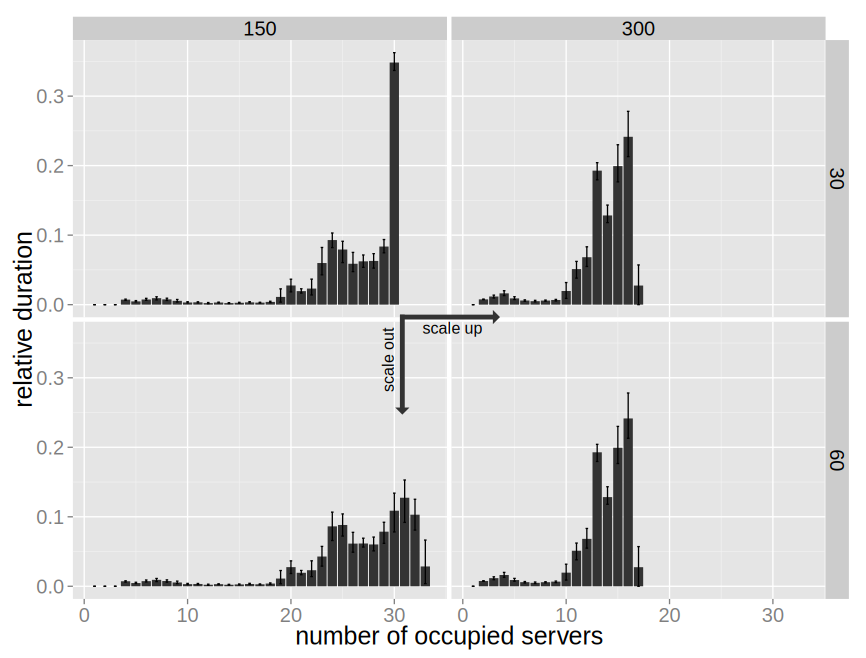
\includegraphics[width=1.0\textwidth]{images/resourceusedistribution-detail-barplot-annotated.pdf}
  \caption{Resource usage from select maximum instances and tunnels combination, displaying the capability to scale.}
 \label{c4:fig:res-usage-barplot}
\end{figure}


\begin{figure}[htb]
  \centering
  \includegraphics[width=1.0\textwidth]{images/startstopduration-blockingprobability-barchart.pdf}
  \caption{Influence of the boot and shutdown time on the blocking probability.}
 \label{c4:fig:blockprob-startstop-barchart}
\end{figure}

\begin{figure}[htb]
  \centering
  \includegraphics[width=1.0\textwidth]{images/feasiblemultiserver-blockprob.pdf}
  \caption{Comparison of the blocking probability of various server configurations.}
 \label{c4:fig:blockprob-multiserver}
\end{figure}

\begin{figure}[htb]
  \centering
  \includegraphics[width=1.0\textwidth]{images/feasiblemultiserver-blockprob.pdf}
  \caption{Comparison of the resource usage of various server configurations.}
 \label{c4:fig:res-usage-multiserver}
\end{figure}

\begin{figure}[htb]
  \centering
  \includegraphics[width=1.0\textwidth]{images/instanceuse-mean.pdf}
  \caption{Mean instance usage of various server configurations.}
 \label{c4:fig:res-instance-usage-mean}
\end{figure}



%%%%%%%%%%%%%%%%%%%%%%%%%%%%%%%%%%%%%%%%%%%%%%%%%%%%%%%%%%%%%%%%%%%%%%%%%%%%%%%
\subsection{Modeling Discussion}






%%%%%%%%%%%%%%%%%%%%%%%%%%%%%%%%%%%%%%%%%%%%%%%%%%%%%%%%%%%%%%%%%%%%%%%%%%%%%%%%
\section{Summary}
\label{c4:sec:conclusion}
In this paper, we take a look at the signaling behavior of devices in an operational \gls{3G} mobile network providing Internet access. Our focus does not lie on the wireless or user-oriented parts of the network, but on signaling in the core network. To the best of our knowledge, this paper is the first to offer a core network perspective on signaling. We give a \gls{GPRS} and \gls{UMTS} network primer, and introduce \gls{GTP} tunnel management, explaining the causes and actions within the network. Our evaluation is based on a week long data set acquired in the core network of an Austrian mobile operator.

% We now go back to the case of Angry Birds which was much quoted for causing excessive radio signaling at one point in time. 
In our observation of core network signaling involving PDP Contexts and their management, we looked at the effect of device types and operating systems on the duration of GTP tunnels. We can conclude that the distribution of tunnel durations in our evaluated dataset is dominated by smartphones. This is contrary to the conventional idea that a larger volume of user plane traffic also leads to an increase of signaling. In our dataset, this would mean that 3G dongles would cause most signaling, which is definitely not the case. In this aspect, our findings support the stories of the casual game ``Angry Birds'' causing signaling storms in mobile networks by frequently downloading small ads, each small download resulting in disproportionate amounts of signaling load being generated. We conjecture from our results that measures taken to improve the radio interface control plane such as Fast Dormancy can have the converse effects in the core, as they could increase the tunnel churn.

All in all, our paper shows that operators can determine which type of device has the most influence on the current network infrastructure by looking at and comparing tunnel duration distributions. %Moreover, if a load situation occurs in the core network, the operator can decide which devices are the root cause and take appropriate measures. 
This investigations can also lead to better network planning that is more aware of the control plane by providing the necessary tools to identify probable causes for control plane activity. Lastly, we hope to raises some awareness with programmers about the potential unintended side effects their application traffic patterns can cause.

\subsection{Future Endeavors}

This paper serves as an introduction to the topic of the 3G core network control plane, and therefore provides only some initial insights into the actual signaling dynamics. Therefore, we would like to expand our evaluations, as there are several  angles not investigated so far that could prove worthwhile.

To get a grasp of the imposed load on the network as well as the involved network nodes, a calculation of the sizes of the tunneling messages was already hinted at. To improve on this naive attempt, actual numbers on the message sizes and involved \glspl{IE} could be recorded in future traces. Having correct signaling traffic volume data still does not reveal the processing load on core network elements. We plan to improve our methodology in this respect by taking at a look at how long it takes for the gateway nodes to process \gls{GTP} messages with respect to the current amount of user traffic and signaling. \gls{GTP} tunnels also cause a certain amount of overhead through additional headers and potential fragmentation of the user traffic, providing another investigation venue for the future (albeit more oriented towards user-plane IP traffic). 

Furthermore, besides the device-based classification, a differentiation based on the user traffic dynamics and correlation to signaling is planned. When looking closer at specific users, the mobility behavior also comes to mind. To investigate this, we intend to take a closer look at the occurring tunnel update messages as evidence, amongst others for mobility.

We also look forward to searching for multiple active tunnels per device. As discussed previously, the \textit{Secondary PDP Context Activation Procedure} enables devices to establish up to ten additional tunnels attributed with a different, higher QoS level, if the network supports this. The additional load of managing and holding multiple tunnels plus the displacement of other, ``lower-quality'' traffic could prove to be an interesting investigation. Initial observations indicate that this feature is rarely used today by very few types of devices, but it will be of increased interest in the face of ongoing LTE/EPS deployments, whose specifications expand upon this secondary tunnel concept.



%%%%%%%%%%%%%%%%%%%%%%%%%%%%%%%%%%%%%%%%%%%%%%%%%%%%%%%%%%%%%%%%%%%%%%%%%%%%%%%%
%%% CoNEXT Conclusion Starts here

In this paper, we took a look at the signaling behavior of devices in an operational \gls{3G} mobile network providing Internet access. Our focus does not lie on the wireless or user-oriented parts of the network, but on signaling in the core network. To the best of our knowledge, this paper is the first to offer an in-depth core network perspective on signaling. We gave a \gls{GPRS} and \gls{UMTS} network primer, and introduced \gls{GTP} tunnel management and evaluated a week long data set recorded in the core network of an Austrian mobile operator.

In our observation of core network signaling involving \gls{PDP} Contexts and their management, we looked at the effect of device types and operating systems on the duration of \gls{GTP} tunnels. We can conclude that the distribution of tunnel durations in our evaluated dataset is dominated by smartphones. This is contrary to the conventional idea that a larger volume of user plane traffic also leads to an increase of signaling. In our dataset, this would mean that 3G dongles would cause most signaling, which is definitely not the case. Our paper shows that operators can determine which type of device has the most influence on the current network infrastructure by looking at and comparing tunnel duration distributions.

For additional load investigations we also looked at the inter-arrival and processing time of tunnels and found further evidence of radio and diurnal effects influencing the core network. With this data in mind, an initial M/M/$\infty$ queue was created to model load occurring at the \gls{GGSN} with simple stationary analysis. This also serves a basis for future more detailed models.

We think that this investigation and load modeling can lead to better network planning: Being more aware of the control plane provides the necessary tools to identify probable causes for control plane activity. We would also like to expand our evaluations, as there are several angles not investigated so far that could prove worthwhile. This includes an examination of the exact number and size of signaling messages flowing through the core, a more detailed picture of the processing load these messages induce at the \gls{GGSN}, and an evolved model. Furthermore, a differential analysis of our data compared to a newer dataset (potentially including \gls{LTE} access) could really prove worthwhile.



%%%%%%%%%%%%%%%%%%%%%%%%%%%%%%%%%%%%%%%%%%%%%%%%%%%%%%%%%%%%%%%%%%%%%%%%%%%%%%%%
%%% MMB2014 Conclusion Starts here
In this paper we investigated trade-offs when virtualizing components of the mobile core network.

To this end, we first discussed a novel approach to mobile core network load modeling based on the control plane load at the \gls{GGSN}. The M/G/$c_c$ loss model is based on the currently implemented state of the network architecture and can serve as a baseline reference to plan and dimension one's own mobile network accordingly, not just based on expected user traffic as traditionally. To improve scaling in the future, we proposed a completely new and virtualizable approach to a \gls{GGSN}'s makeup.

Then, we presented random variables to model load in a \gls{GGSN} based on measurement data from the network of a nation-wide mobile service provider and made them available for reuse by other researchers.

Finally, we evaluate the model using a queing simulation. We have shown, that the system's blocking probability is roughly equal to the single-server model but in addition achieves large efficiency gains, even with very simplistic provisioning conditions and very long boot times. The model also has the ability to very easily scale out one's infrastructure by simply adding more small servers, reducing operational overhead. This might even lead to a new GGSN-as-a-Service business models, removing the need to provide and operate large amounts of infrastructure for rare cases of peak load. 
In the future we would like to deepen our modeling efforts to provide more dimensioning options for a core network. Also, we want to further investigate the correlation of user traffic and signaling and take a look at the implications specific traffic types bring for the core network. 